\documentclass[conference]{IEEEtran}
\usepackage{silence}
\WarningFilter{caption}{Unknown document class}
\WarningFilter{latex}{Text page}
\usepackage{cite}
\usepackage{amsmath,amssymb,amsfonts,amsthm}
\usepackage{xcolor}
\usepackage{graphicx}
\usepackage{tikz}
\usetikzlibrary{positioning,arrows.meta,shapes.geometric,calc}
\usepackage{booktabs}
\usepackage{longtable}
\usepackage{subcaption}
\captionsetup{compatibility=false}
\usepackage{algorithm}
\usepackage{algpseudocode}
\usepackage{array}
\usepackage{multirow}
\usepackage{makecell}
\usepackage{tabularx}
\usepackage{bookmark}
\usepackage{xurl}
\usepackage{hyperref}
\usepackage{float}
\newtheorem{proposition}{Proposition}
\newtheorem{remark}{Remark}
\tikzset{
  flow/.style={-Latex, line width=1.0pt, draw=black},
  every node/.style={anchor=center}
}
\urlstyle{same}
\hypersetup{hidelinks,pdfcreator={LaTeX via pandoc}}
\makeatletter
\def\maxwidth{\ifdim\Gin@nat@width>\linewidth\linewidth\else\Gin@nat@width\fi}
\def\maxheight{\ifdim\Gin@nat@height>\textheight\textheight\else\Gin@nat@height\fi}
\makeatother
\setkeys{Gin}{width=\maxwidth,height=\maxheight,keepaspectratio}
\setlength{\emergencystretch}{3em}

\author{\IEEEauthorblockN{Yingjie Zhang}
\IEEEauthorblockA{\textit{School of Computer Science}\\
\textit{Guangdong University of Technology}\\
Guangzhou, China}
\and
\IEEEauthorblockN{Xiao-Min Hu \textsuperscript{*}}
\IEEEauthorblockA{\textit{School of Computer Science} \\
\textit{Guangdong University of Technology}\\
Guangzhou, China \\
*Corresponding Author: xmhu@gdut.edu.cn}
\and
\IEEEauthorblockN{Jing-Chuan Tang}
\IEEEauthorblockA{\textit{School of Computer Science} \\
\textit{Guangdong University of Technology}\\
Guangzhou, China}
}

\begin{document}

\title{Conflict-Gated Communication for Distributed Black-Box Optimization:\\When to Negotiate Under a Communication Budget}
\maketitle

\begin{abstract}
Network-based distributed optimization (NDO) with mixed private and shared variables must repeatedly coordinate neighbors on shared dimensions, yet always-on negotiation wastes communication when local conflict is weak or stale. This paper treats \emph{communication timing}, the decision of whether to open the negotiation channel at each outer loop, as a first-class problem rather than a fixed rule inside one algorithm. We propose \emph{conflict-triggered communication}. A cheap online conflict proxy triggers negotiation only when inconsistency exceeds a phase-relative baseline, and a fail-safe period guarantees non-zero communication so consensus references do not freeze. The policy is instantiated on the MACPO penalty-negotiation backbone and tested on the MACPO NDO benchmark (F1--F18), periodic-communication baselines, gate ablations, MACPO-style dispatch simulators, and IEEE transmission-network pilots. Conflict gating cuts negotiation trigger rates from always-on to a small fraction of outer loops while preserving or improving final fitness under identical evaluation budgets. Penalty-controller choice (RL, EMA, or fixed schedules) is secondary once gating is fixed. The same mechanism transfers to communication-constrained economic dispatch.
\end{abstract}

\begin{IEEEkeywords}
distributed black-box optimization, communication timing, event-triggered coordination, conflict gating, network-based optimization, economic dispatch
\end{IEEEkeywords}

\section{Introduction}\label{sec:intro}
Network-based distributed optimization (NDO) models systems in which many agents on a graph optimize a global objective through local information and neighbor interaction \cite{ref_bertsekas_tsitsiklis,ref_decentralized_review_2023}. A defining feature is the mixture of private variables and shared edge-coupled variables. When objectives are black-box and only locally evaluable, coordination must proceed without analytic gradients, through repeated local search and neighbor negotiation on shared dimensions.

Penalty-based cooperative evolution, exemplified by MACPO \cite{ref_macpo}, is a practical NDO backbone: each agent optimizes a penalized local objective and negotiates with neighbors to align shared variables. MACPO opens communication on nearly every outer loop. When conflict is weak, this cost may not improve shared-variable consistency or final fitness. The bottleneck is therefore not only \emph{how} to negotiate, but \emph{when} negotiation is worth its communication and evaluation cost.

This paper addresses the \textbf{communication-timing problem in distributed black-box optimization}. At each outer iteration, should agents open the negotiation channel? We answer with \textbf{conflict-triggered communication}, a rule-based gate driven by an online conflict proxy, a relative threshold, and a fail-safe silent bound. The gate is orthogonal to the specific penalty or local optimizer. MACPO serves as the reference instantiation and engineering platform, not as the conceptual endpoint.

Three research lines motivate this formulation. In communication-efficient distributed optimization, Local SGD and FedAvg reduce gradient-exchange frequency while retaining convergence under smoothness assumptions \cite{ref_stich_local_sgd_2019,ref_mcmahan_fedavg_2017,ref_koloskova_decsgd_2020}. In event-triggered and self-triggered control, agents communicate when a local error signal crosses a threshold rather than at every clock tick \cite{ref_rabbat_nowak_2004}. In distributed black-box NDO, MACPO \cite{ref_macpo}, MASOIE \cite{ref_masoie_2024}, and MAES-CCSA \cite{ref_maes_ccsa_2025} adapt coordination schedules but do not jointly formalize \emph{when}-to-communicate as an explicit decision with a controllable communication--quality trade-off. Our contribution fills that gap for penalty-negotiation NDO.

The contributions are:
\begin{enumerate}
\item \textbf{Problem formulation.} Communication timing in NDO is cast as a per-iteration binary scheduling decision under a communication budget or fitness tolerance (Section~\ref{sec:timing_problem}).
\item \textbf{Conflict-triggered gate.} A three-layer gate (minimum interval, relative conflict threshold, fail-safe bound) with structural propositions on silent-period limits and skippable low-conflict rounds (Section~\ref{sec:gate_design}).
\item \textbf{Empirical validation on three axes.} Route~1 covers benchmark and mechanism studies on F1--F18 with periodic and gate ablations. Route~2 covers MACPO-style dispatch and IEEE pilots under bandwidth-limited coordination. Route~3 reports that adaptive penalty control is a plug-in interface, not the dominant gain (Sections~\ref{sec:experiments}--\ref{sec:applications}).
\end{enumerate}

\section{Related Work and Positioning}\label{sec:related}
Gradient-based distributed methods---DGD, ADMM, EXTRA, Push--Pull---provide strong guarantees when objectives are convex and gradients exist \cite{ref_nedic_subgrad,ref_boyd_admm,ref_shi_extra,ref_pu_pushpull_2021}. They are less directly applicable to black-box NDO with explicit shared-variable negotiation \cite{ref_back_book,ref_blackbox_tracking_2022}. Cooperative coevolution and penalty methods offer a gradient-free path \cite{ref_potter_dejong,ref_cc_dist_accel_2024,ref_macpo} but typically treat communication as fixed.

Table~\ref{tab:positioning} places our work in the communication-efficiency spectrum. MACPO is the structural backbone. MASOIE and MAES-CCSA are recent distributed black-box competitors with adaptive intervals or step rules. We compare against always-on MACPO, periodic-$K$ communication, and internal gate variants. External black-box baselines remain a stated limitation.

\begin{table}[!t]
\centering
\scriptsize
\caption{Positioning of conflict-triggered communication in the communication-efficiency landscape.}
\label{tab:positioning}
\setlength{\tabcolsep}{3pt}
\begin{tabular}{@{}p{0.19\columnwidth}p{0.22\columnwidth}p{0.24\columnwidth}p{0.25\columnwidth}@{}}
\toprule
\textbf{Line} & \textbf{Trigger signal} & \textbf{Typical setting} & \textbf{Relation to this work} \\
\midrule
Periodic comm. & Fixed clock / interval & Local SGD, FedAvg & Baseline schedule, no conflict feedback \\
Event-triggered & Error vs.\ threshold & Control, sensor nets & Same philosophy, black-box CI proxy \\
MACPO & Implicit (every loop) & Penalty NDO & Backbone, always-on status quo \\
MASOIE / MAES-CCSA & Stage / path consistency & DBO swarms & Different topology, spectrum neighbors \\
\textbf{Ours} & Relative CI + fail-safe & Penalty-negotiation NDO & Explicit timing + trade-off control \\
\bottomrule
\end{tabular}
\end{table}

Reinforcement learning appears in metaheuristic parameter control \cite{ref_karafotias_param_control,ref_rl_ea_survey_2024}. In our instantiation, RL is one implementation of the penalty interface. Experiments show it is not necessary once conflict gating is fixed (Section~\ref{sec:q3_penalty}). Future work may apply learning to harder timing decisions such as neighbor or topology selection (Section~\ref{sec:future_rl}).

\section{NDO Formulation}\label{sec:problem}
Consider $n$ agents on an undirected graph $G=(V,E)$ with global decision vector $\mathbf{X}=[x_1,\ldots,x_D]$. For agent $i$,
\begin{equation}
X_i = \mathrm{col}\{x_d\}_{d \in \Theta_i}, \quad \Theta_i = I_i \cup \bigcup_{j \in N_i} I_{i,j}
\label{eq:local_variable_set}
\end{equation}
where $I_i$ indexes private variables on vertex $i$, $I_{i,j}$ indexes shared variables on edge $(i,j)$, and $N_i$ is the neighbor set. The global objective is
\begin{equation}
\min_{X\in\mathbb{R}^D} F(X) = \sum_{i=1}^{n} f_i(X_i)
\label{eq:global_objective}
\end{equation}
subject to $x_i^d = x_j^d$ for all $d\in I_{i,j}$ and $(i,j)\in E$.

\section{The Communication-Timing Problem}\label{sec:timing_problem}
Let $t=1,2,\ldots,T$ index outer iterations. At each $t$, the system chooses a gate $g^t\in\{0,1\}$: if $g^t=1$, agents enter the negotiation branch; if $g^t=0$, they skip negotiation and continue local search while refreshing consensus references. MACPO fixes $g^t\equiv 1$. The communication-timing problem is to design a policy $\pi$ such that $g^t=\pi(\mathcal{H}^t)$, where $\mathcal{H}^t$ contains observable local history (local best, consensus reference, conflict proxy, time since last communication).

Two equivalent objectives capture the engineering trade-off:
\begin{itemize}
\item \textbf{Budget form:} minimize $F(X^T)$ subject to average trigger rate $\bar p_{\mathrm{comm}}=\frac{1}{T}\sum_t g^t \le B$;
\item \textbf{Tolerance form:} minimize $\bar p_{\mathrm{comm}}$ subject to $F(X^T)$ not worse than an always-on baseline by more than tolerance $\delta$.
\end{itemize}
Black-box NDO lacks convexity, so we do not claim global convergence theorems. Instead, we provide \emph{operational sufficient conditions} for skipping communication and \emph{structural bounds} on silent periods, validated empirically (Section~\ref{sec:gate_design}).

\section{Conflict-Triggered Communication}\label{sec:gate_design}
\subsection{Gate Design}
Conflict gating decides \emph{whether} to open communication before paying negotiation cost. Let $\mathrm{CI}_i^t$ be a black-box conflict proxy: the mean normalized discrepancy between the local best and the consensus reference on active overlap dimensions (motivated by the gradient-based conflict index in \cite{ref_macpo}, but computed without gradients). Let $\hat{\mu}_{\mathrm{CI},i}^t$ be its phase EMA baseline. The local gate is
\begin{equation}
g_i^t=\mathbf{1}\left[\mathcal{C}_{\mathrm{int}}^t\land \mathcal{C}_{\mathrm{thr}}^t\land \mathcal{C}_{\mathrm{phase}}^t\right]
\label{eq:local_gate}
\end{equation}
with minimum-interval constraint $\mathcal{C}_{\mathrm{int}}^t$, threshold constraint
$\mathcal{C}_{\mathrm{thr}}^t: \mathrm{CI}_i^t > \lambda\,\hat{\mu}_{\mathrm{CI},i}^t\ \text{or}\ t-t_{\mathrm{last\_comm}}\ge K$,
and phase-sampling constraint $\mathcal{C}_{\mathrm{phase}}^t: u_i^t < p_{\mathrm{phase}}^t$. Global synchronization uses $g_{\mathrm{global}}^t=\max_i g_i^t$ (Eq.~\eqref{eq:global_gate}). Algorithm~\ref{alg:ci_gating} summarizes the procedure.

\begin{equation}
g_{\mathrm{global}}^t=\max_i g_i^t
\label{eq:global_gate}
\end{equation}

\begin{algorithm}[t]
  \footnotesize
  \caption{Conflict-Gated Communication with Phase Sampling}
  \label{alg:ci_gating}
  \begin{algorithmic}[1]
  \For{each outer iteration $t$}
    \State Compute $\mathrm{CI}_i^t$ and update $\hat{\mu}_{\mathrm{CI},i}^t$
    \State Check $\mathcal{C}_{\mathrm{int}}^t$, $\mathcal{C}_{\mathrm{thr}}^t$ (relative threshold or fail-safe $K$), and $\mathcal{C}_{\mathrm{phase}}^t$
    \State $g_i^t\gets \mathbf{1}[\mathcal{C}_{\mathrm{int}}^t\land \mathcal{C}_{\mathrm{thr}}^t\land \mathcal{C}_{\mathrm{phase}}^t]$
    \State $g_{\mathrm{global}}^t\gets \max_i g_i^t$
    \If{$g_{\mathrm{global}}^t=0$} \State Skip negotiation; refresh consensus reference
    \Else \State Enter negotiation branch \EndIf
  \EndFor
  \end{algorithmic}
\end{algorithm}

\subsection{Structural Propositions}
\begin{proposition}[Fail-safe communication lower bound]\label{prop:failsafe}
If $\mathcal{C}_{\mathrm{thr}}^t$ includes fail-safe $t-t_{\mathrm{last\_comm}}\ge K$ and phase sampling satisfies $p_{\mathrm{phase}}^t>0$ on an infinite horizon, then
$\liminf_{T\to\infty}\frac{1}{T}\sum_{t=1}^T g^t \ge 1/K$ up to the phase-sampling floor.
\end{proposition}
\begin{remark}
This prevents unbounded silent periods that freeze consensus references. Empirically, F3--F18 exhibit trigger rates near one negotiation every twelve outer loops under shared defaults (Section~\ref{sec:exp_q2}), consistent with fail-safe/phase paths rather than ad hoc rate caps.
\end{remark}

\begin{proposition}[Skippable low-conflict round (operational)]\label{prop:skip}
Suppose at iteration $t$: (i) $\mathrm{CI}_i^t \le \lambda\hat{\mu}_{\mathrm{CI},i}^t$ for all active agents; (ii) overlap variables moved little since $t_{\mathrm{last\_comm}}$; and (iii) fail-safe has not fired. Then an additional MACPO negotiation round at $t$ yields negligible marginal improvement in logged $f_{\mathrm{pure}}$ relative to skipping, in the sense validated by gate ablations, CI-conditioned trigger statistics (Fig.~\ref{fig:ci_bin_trigger}), and communication summaries (Tables~\ref{tab:gate_cost_stats},~\ref{tab:f1f6_comm_eva}).
\end{proposition}
\begin{remark}
This is an operational sufficient condition, not a MACPO convergence theorem. It aligns with event-triggered control: communicate when the error signal is informative. Fig.~\ref{fig:comm_fitness_pareto} shows gated policies occupy a better communication--fitness region than fixed-interval schedules on F1/F2/F5; Fig.~\ref{fig:ci_bin_trigger} shows that empirical trigger probability is not uniform across conflict quantiles---mid/low-conflict bins trigger less often than the lowest quintile, where fail-safe and interval paths dominate (Proposition~\ref{prop:failsafe}).
\end{remark}

\subsection{Expected Communication--Quality Trade-off}
Under gate $g^t$, expected negotiation cost scales as $\mathcal{O}(I\,\bar p_{\mathrm{comm}}\,\bar r_{\mathrm{act}}\sum_{(i,j)}|L_{i,j}|)$ versus $\mathcal{O}(I\sum_{(i,j)}|L_{i,j}|)$ for always-on MACPO (Section~\ref{sec:complexity}). Knobs $(\lambda,K,p_{\mathrm{phase}})$ trace a controllable trade-off surface between $\bar p_{\mathrm{comm}}$ and terminal $F$.

\section{MACPO Instantiation}\label{sec:method}
We instantiate conflict-triggered communication on the MACPO backbone \cite{ref_macpo}. Each agent optimizes $h_i(x)=f_i(x)+\alpha_i c_i(x)$ locally, then---if $g_{\mathrm{global}}^t=1$---negotiates on shared variables via Nash-style competition and two-sided perturbation checking (Algorithm~\ref{alg:negotiation_consistency}). Fig.~\ref{fig:rl_macpo_architecture} shows the pipeline; \emph{communication} is the gate decision, \emph{negotiation} is post-gate processing.

\begin{figure*}[htbp]
\centering
\begin{subfigure}[t]{0.66\textwidth}
\centering
\resizebox{\linewidth}{!}{%
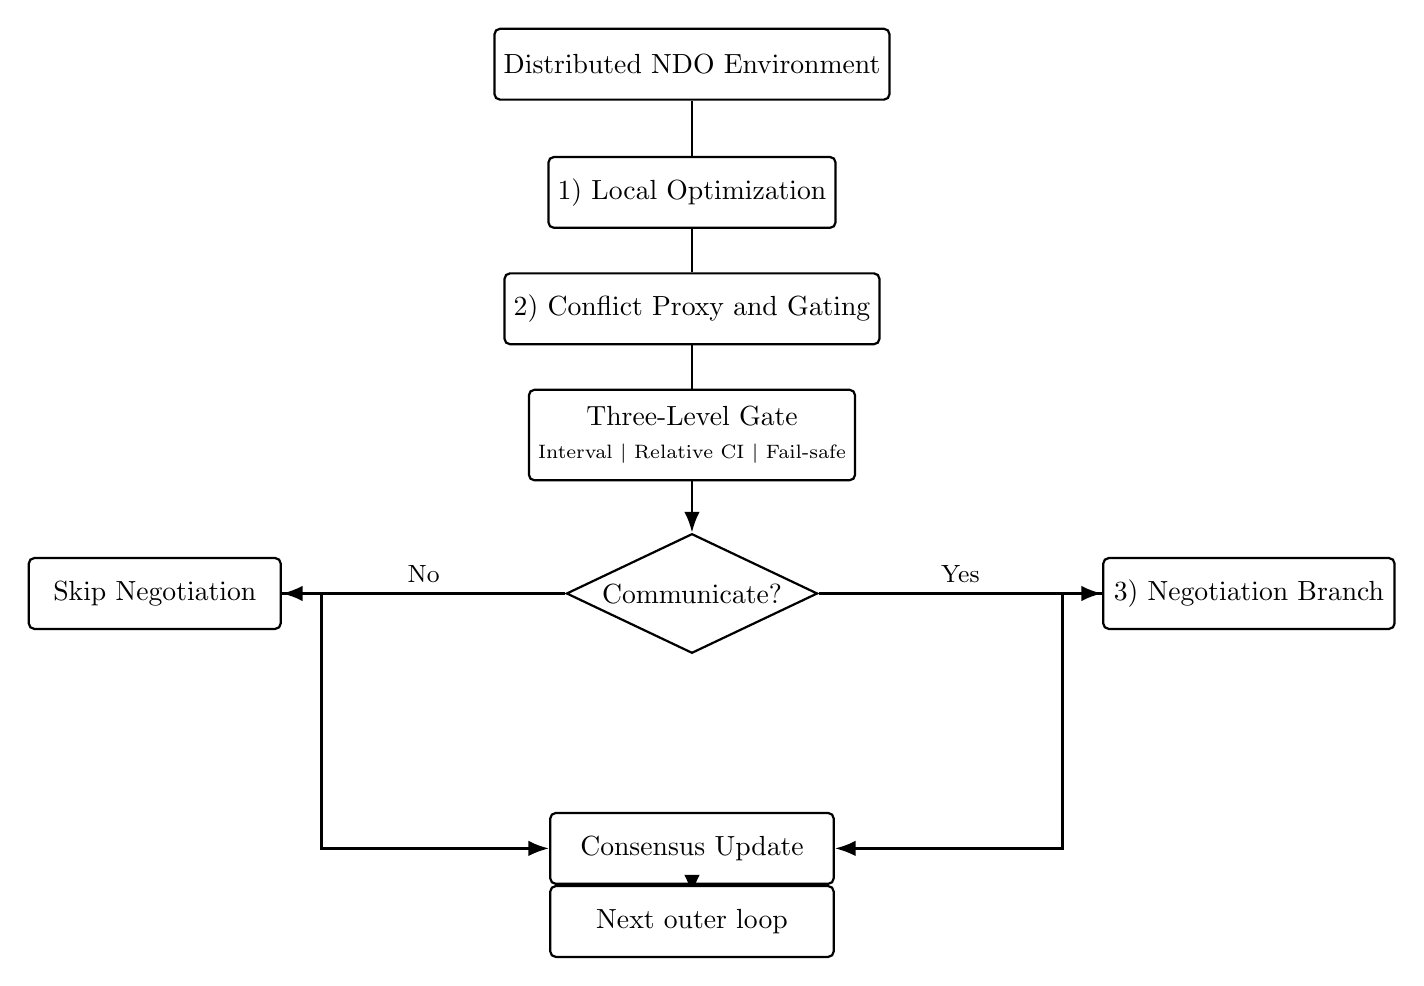
\begin{tikzpicture}[
  font=\normalsize,
  line/.style={-Latex, line width=1.0pt, draw=black},
  box/.style={rounded corners=2pt, draw=black, fill=white, line width=0.8pt, minimum width=3.6cm, minimum height=0.90cm, align=center},
  flow/.style={box},
  gate/.style={box, minimum width=4.1cm, minimum height=1.15cm},
  nego/.style={box, minimum width=3.7cm},
  skip/.style={box, minimum width=3.2cm},
  decision/.style={diamond, draw=black, fill=white, line width=0.8pt, aspect=2.1, inner sep=1.8pt, align=center}
]
\node[flow] (env) at (0,5.7) {Distributed NDO Environment};
\node[flow, below=0.70cm of env] (opt) {1) Local Optimization};
\node[flow, below=0.55cm of opt] (conf) {2) Conflict Proxy and Gating};
\node[gate, below=0.55cm of conf] (gating) {Three-Level Gate\\{\scriptsize Interval $\mid$ Relative CI $\mid$ Fail-safe}};
\node[decision, below=0.65cm of gating] (decide) {Communicate?};
\node[nego, right=3.6cm of decide] (ex) {3) Negotiation Branch};
\node[skip, left=3.6cm of decide] (skp) {Skip Negotiation};
\node[flow, below=2.0cm of decide] (cons) {Consensus Update};
\draw[line] (env) -- (opt) -- (conf) -- (gating) -- (decide);
\draw[line] (decide.east) -- node[above, font=\small] {Yes} (ex.west);
\draw[line] (decide.west) -- node[above, font=\small] {No} (skp.east);
\draw[line] (ex.west) -- ++(-0.5cm,0) |- (cons.east);
\draw[line] (skp.east) -- ++(0.5cm,0) |- (cons.west);
\draw[line] (cons) -- ++(0,-0.6) node[flow, below=0cm of cons] (loop) {Next outer loop};
\end{tikzpicture}%
}
\caption{Conflict-triggered MACPO pipeline. Gating is the primary design lever.}
\label{fig:rl_macpo_main}
\end{subfigure}
\hfill
\begin{subfigure}[t]{0.30\textwidth}
\centering
\includegraphics[width=\linewidth]{media/image_rl_penalty_loop.png}
\caption{Optional penalty interface (RL default).}
\label{fig:rl_macpo_rl}
\end{subfigure}
\caption{Instantiation on MACPO: conflict gating (a) is the core mechanism; adaptive penalty (b) is a plug-in module.}
\label{fig:rl_macpo_architecture}
\end{figure*}

\begin{algorithm}[t]
  \footnotesize
  \caption{Negotiation with Two-Sided Consistency Check (Abstract)}
  \label{alg:negotiation_consistency}
  \begin{algorithmic}[1]
  \Require Neighbor pair $(i,j)$, shared set $L_{i,j}$, variable switch $\mathrm{switch}[\cdot]$
  \For{each shared dimension $d\in L_{i,j}$ with $\mathrm{switch}[d]=1$}
    \State Nash-style bilateral comparison on $d$
    \State Two-sided perturbation check; update $\mathrm{switch}[d]$ if consistent
    \State Write accepted values to consensus reference
  \EndFor
  \State Re-evaluate local population
  \end{algorithmic}
\end{algorithm}

\subsection{Optional Modules (Secondary)}\label{sec:optional_modules}
\textbf{Variable selection.} Once communication is granted, shared dimensions can be ranked by importance score $q_d^t$; low-impact dimensions may be skipped. Ablations show this is auxiliary once gating is active (Section~\ref{sec:q3_modules}).

\textbf{Adaptive penalty interface (Route~3).}\label{sec:penalty_interface}
Penalty strength adapts through a common interface (RL default, EMA, or fixed phase schedules). Under fixed gating, controllers are statistically tied on F3/F5 (Table~\ref{tab:penalty_controller_f3_f5}); RL is retained as a unified default without benchmark-specific schedules, not as a universal superiority claim.

\section{Experimental Evaluation}\label{sec:experiments}
We organize experiments around four questions aligned with the communication-timing formulation:
\begin{itemize}
\item \textbf{Q1 (Quality):} Does gated MACPO match or improve fitness at the same evaluation budget?
\item \textbf{Q2 (Communication):} Does conflict triggering reduce $\bar p_{\mathrm{comm}}$ without sacrificing Q1?
\item \textbf{Q3 (Mechanism):} Is gating necessary? Is RL necessary once gating is fixed?
\item \textbf{Q4 (Transfer):} Does the mechanism transfer to dispatch and grid pilots (Route~2)?
\end{itemize}
Protocol: MACPO NDO suite F1--F18 \cite{ref_macpo}, 25 paired runs, LLSO primary and CSO secondary, Wilcoxon/Mann--Whitney tests at the conventional 0.05 level. Table columns use \textbf{RL-MACPO} for the archived implementation name (full stack with conflict gate; RL penalty default unless an ablation caption states otherwise).

\subsection{Experimental Setup}
\paragraph{Benchmark.} We use the MACPO NDO suite F1--F18 \cite{ref_macpo} under the \emph{Full} RL-MACPO configuration unless an ablation caption states otherwise. Dispatch and IEEE cases are in Section~\ref{sec:applications}. Table~\ref{tab:benchmark_f1f6} lists the primary small-scale chain family (20 agents, $D{=}905$). Homogeneous instances F1--F3 share one base landscape per agent. Heterogeneous instances F4--F6 mix elliptic, Schwefel, and Rosenbrock segments. Theory CI in the table is the average conflict index from \cite{ref_macpo}. RL-MACPO uses a black-box conflict proxy in the same role for gating. By theory CI, F3 and F5 are high-conflict (0.846 and 0.497), F2 and F4 are low-conflict (0.049 and 0.051), and F1 and F6 are mid-range (0.228 and 0.268).

\begin{table}[!t]
\centering
\small
\caption{MACPO small-scale benchmark family F1--F6 (20-agent chain, $D{=}905$). F1--F3 are homogeneous; F4--F6 are heterogeneous \cite{ref_macpo}.}
\label{tab:benchmark_f1f6}
\begin{tabular}{@{}lll@{}}
\toprule
\textbf{Func.} & \textbf{Composition} & \textbf{Theory CI} \\
\midrule
\multicolumn{3}{@{}l}{\textit{Homogeneous}} \\
F1 & Elliptic & 0.228 \\
F2 & Schwefel & 0.049 \\
F3 & Rosenbrock & 0.846 \\
\addlinespace[0.15em]
\multicolumn{3}{@{}l}{\textit{Heterogeneous}} \\
F4 & Elliptic--Schwefel & 0.051 \\
F5 & Elliptic--Rosenbrock & 0.497 \\
F6 & Schwefel--Rosenbrock & 0.268 \\
\bottomrule
\end{tabular}
\end{table}

\paragraph{Evaluation protocol.} MACPO and RL-MACPO share paired seeds, the MACPO evaluation-budget cap, and embedded optimizers LLSO \cite{ref_llso} (primary) and CSO \cite{ref_cso} (secondary). End-of-run evaluation counts differ by at most a few percent (Table~\ref{tab:f1f6_comm_eva}); indicative wall-clock overhead is reported separately (Table~\ref{tab:wall_time_f1_f18}) and is not used as a primary endpoint.

\paragraph{Notation and statistics.} $F(\mathbf{X})$ denotes the global objective in Eq.~\eqref{eq:global_objective}. Logged $f_{\mathrm{pure}}$ is the pure objective sum without penalty terms; $f_{\mathrm{penalty}}$ includes conflict penalties. Lower is better unless a caption states otherwise. Main tables report mean, median, standard deviation, and win/tie/loss over \textbf{25 independent runs}. RL-MACPO vs.\ MACPO uses paired Wilcoxon signed-rank tests (LLSO) or Mann--Whitney U tests (CSO) at the conventional 0.05 significance level \cite{ref_macpo}. Boldface marks the better mean within each MACPO vs.\ RL-MACPO pair; * and \# denote significance in Table~\ref{tab:macpo_style_all}.

\subsection{Experimental Roadmap}\label{sec:exp_roadmap}
The evaluation is organized around four questions tied to the communication-efficiency goal of Section~\ref{sec:intro}. Fig.~\ref{fig:exp_roadmap} shows the reading order; the four blocks below state what each question tests and where the evidence appears.

\begin{figure}[!t]
\centering
\resizebox{\columnwidth}{!}{%
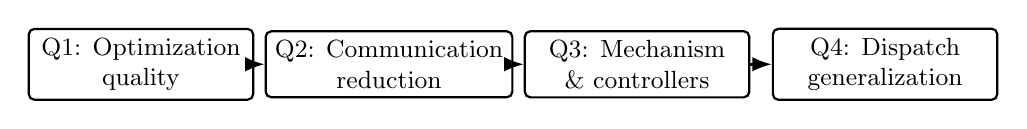
\begin{tikzpicture}[
  font=\small,
  box/.style={draw, rounded corners=2pt, line width=0.8pt, minimum width=2.85cm, minimum height=0.72cm, align=center, fill=white},
  arr/.style={-Latex, line width=0.9pt, draw=black}
]
\node[box] (q1) at (0,0) {Q1: Optimization\\quality};
\node[box] (q2) at (3.15,0) {Q2: Communication\\reduction};
\node[box] (q3) at (6.3,0) {Q3: Mechanism\\ \& controllers};
\node[box] (q4) at (9.45,0) {Q4: Dispatch\\generalization};
\draw[arr] (q1.east) -- (q2.west);
\draw[arr] (q2.east) -- (q3.west);
\draw[arr] (q3.east) -- (q4.west);
\end{tikzpicture}%
}
\caption{Experimental roadmap (left to right). Details for each block are in the text below.}
\label{fig:exp_roadmap}
\end{figure}

\paragraph{Q1 (Optimization quality).}
Does RL-MACPO match or improve final fitness under the \emph{same} evaluation budget as MACPO? We compare paired 25-run batches on F1--F18 with LLSO (primary) and CSO (secondary), reporting mean, median, standard deviation, and significance (Tables~\ref{tab:macpo_style_all} and~\ref{tab:macpo_rl_mean_f1_f18}; convergence curves in Fig.~\ref{fig:fes_f1_f6_panel}).

\paragraph{Q2 (Communication reduction).}
Can conflict-gated communication cut negotiation rate without sacrificing Q1 fitness? We report outer-loop trigger rates, evaluation-budget parity, gate-variant diagnostics, CI-bin trigger statistics (Fig.~\ref{fig:ci_bin_trigger}), and a communication--fitness trade-off (Tables~\ref{tab:f1f6_comm_eva},~\ref{tab:comm_rate_f1_f18}, and~\ref{tab:gate_cost_stats}; Fig.~\ref{fig:comm_fitness_pareto}).

\paragraph{Q3 (Mechanisms and controllers).}
Which modules matter, and is RL necessary once gating is fixed? Section~\ref{sec:q3_penalty} compares RL, EMA, and fixed penalty schedules on F3/F5 under identical gating; Section~\ref{sec:q3_modules} ablates gating layers, variable selection, phase sampling, and $\eta$ strategies (Table~\ref{tab:penalty_controller_f3_f5}, Fig.~\ref{fig:gating_ablation}, Tables~\ref{tab:deeprl} and~\ref{tab:phase_eta}).

\paragraph{Q4 (Dispatch generalization).}
Do benchmark savings transfer to MACPO-style dispatch simulators and IEEE transmission-network pilots? Section~\ref{sec:applications} reports paired communication rate and pure-objective change on application cases and IEEE~30/57/118 (Tables~\ref{tab:application_cases} and~\ref{tab:ieee_power_cases}).

\subsection{Question 1: Does RL-MACPO Preserve Optimization Quality?}\label{sec:exp_q1}
To answer whether RL-MACPO improves final fitness under the same evaluation budget as MACPO, we compare paired 25-run batches on F1--F18 (Tables~\ref{tab:macpo_style_all},~\ref{tab:macpo_rl_mean_f1_f18}; Fig.~\ref{fig:fes_f1_f6_panel}). Table~\ref{tab:macpo_style_all} also lists \emph{RL Only} (adaptive penalty without gating) for reference; GFPDO$^{\dagger}$/DPSO$^{\dagger}$ columns follow the MACPO paper layout \cite{ref_macpo} without significance tests.

\begin{table*}[!t]
\centering
\tiny
\setlength{\tabcolsep}{1.8pt}
\renewcommand{\arraystretch}{1.00}
\caption{Final global objective $F$ (Eq.~\protect\eqref{eq:global_objective}) on F1--F6: mean, median, standard deviation, and $p$-value over 25 independent runs, for LLSO (left five columns) and CSO (right five columns). \textbf{MACPO} and \textbf{RL-MACPO} use logged $f_{\mathrm{pure}}$ (last row per run) from archived trajectories. \textbf{GFPDO$^{\dagger}$}: one-run pilot per function under the MACPO GFPDO executable; \textbf{DPSO$^{\dagger}$}: 25-run batch under the MACPO DPSO executable (same evaluation budget). No significance tests for external columns. Tests for RL-MACPO vs.\ MACPO only: paired Wilcoxon signed-rank (LLSO), Mann--Whitney U (CSO). * RL-MACPO better; \# worse (significant at the 0.05 level). Bold: better mean in each MACPO vs.\ RL-MACPO pair.}
\label{tab:macpo_style_all}
\resizebox{\textwidth}{!}{%
\begin{tabular}{llccccc|ccccc}
\toprule
\multirow{2}{*}{\makecell[c]{\textbf{Bench.}}} & \multirow{2}{*}{\textbf{Metric}} & \multicolumn{5}{c}{\textbf{LLSO}} & \multicolumn{5}{c}{\textbf{CSO}} \\
\cmidrule(lr){3-7}\cmidrule(lr){8-12}
& & \textbf{GFPDO$^{\dagger}$} & \textbf{DPSO$^{\dagger}$} & \textbf{MACPO} & \textbf{RL Only} & \textbf{RL-MACPO} & \textbf{GFPDO$^{\dagger}$} & \textbf{DPSO$^{\dagger}$} & \textbf{MACPO} & \textbf{RL Only} & \textbf{RL-MACPO} \\
\midrule
\multirow{4}{*}{F1}
& mean    & 3.00E+9 & 4.57E+10 & 1.98E+7 & 2.07E+7 & \textbf{6.43E+6} & 4.73E+10 & 8.84E+10 & 2.33E+7 & 2.02E+7 & \textbf{1.25E+7} \\
& median  & 3.00E+9 & 4.65E+10 & 2.00E+7 & 1.97E+7 & \textbf{6.48E+6} & 4.73E+10 & 8.82E+10 & 2.24E+7 & 2.00E+7 & \textbf{1.27E+7} \\
& std     & 0 & 4.82E+9 & 1.71E+6 & 3.58E+6 & \textbf{3.52E+5} & 0 & 4.27E+9 & 2.98E+6 & 1.34E+6 & \textbf{6.26E+5} \\
& p-value & --- & --- & - & 5.46e-01 & 2.98e-08* & --- & --- & - & 2.41e-05* & 6.90e-10* \\
\midrule
\multirow{4}{*}{F2}
& mean    & 2.20E+7 & 6.82E+9 & 5.05E+4 & 4.76E+4 & \textbf{3.32E+3} & 1.61E+10 & 1.55E+11 & 6.95E+4 & 6.43E+4 & \textbf{9.11E+3} \\
& median  & 2.20E+7 & 6.98E+9 & 4.83E+4 & 4.35E+4 & \textbf{3.33E+3} & 1.61E+10 & 1.49E+11 & 6.81E+4 & 6.38E+4 & \textbf{9.09E+3} \\
& std     & 0 & 3.13E+9 & 6.23E+3 & 9.67E+3 & \textbf{1.33E+2} & 0 & 4.84E+10 & 5.90E+3 & 6.98E+3 & \textbf{8.06E+2} \\
& p-value & --- & --- & - & 5.46e-01 & 2.98e-08* & --- & --- & - & 2.41e-05* & 7.07e-10* \\
\midrule
\multirow{4}{*}{F3}
& mean    & 6.07E+10 & 2.19E+11 & 4.03E+9 & 5.89E+9 & \textbf{6.35E+2} & 3.36E+11 & 6.08E+11 & 1.51E+9 & 2.66E+9 & \textbf{6.70E+2} \\
& median  & 6.07E+10 & 2.18E+11 & 4.05E+9 & 5.86E+9 & \textbf{6.32E+2} & 3.36E+11 & 6.00E+11 & 1.51E+9 & 2.60E+9 & \textbf{6.45E+2} \\
& std     & 0 & 4.54E+9 & 4.79E+8 & 7.13E+8 & \textbf{3.12E+1} & 0 & 3.64E+10 & 8.57E+7 & 2.64E+8 & \textbf{2.63E+2} \\
& p-value & --- & --- & - & 5.46e-01 & 2.98e-08* & --- & --- & - & 2.41e-05* & 6.98e-10* \\
\midrule
\multirow{4}{*}{F4}
& mean    & 9.28E+8 & 2.43E+10 & 3.17E+6 & 3.01E+6 & \textbf{2.58E+6} & 3.09E+10 & 6.35E+10 & 7.30E+6 & 6.98E+6 & \textbf{5.80E+6} \\
& median  & 9.28E+8 & 2.42E+10 & 3.14E+6 & 2.98E+6 & \textbf{2.61E+6} & 3.09E+10 & 6.14E+10 & 7.16E+6 & 6.90E+6 & \textbf{5.80E+6} \\
& std     & 0 & 3.32E+9 & 3.59E+5 & 2.71E+5 & \textbf{1.29E+5} & 0 & 6.59E+9 & 7.53E+5 & 9.53E+5 & \textbf{3.82E+5} \\
& p-value & --- & --- & - & 5.46e-01 & 8.94e-08* & --- & --- & - & 2.41e-05* & 1.82e-09* \\
\midrule
\multirow{4}{*}{F5}
& mean    & 2.67E+10 & 8.55E+10 & 1.97E+8 & 4.24E+8 & \textbf{3.50E+6} & 1.45E+11 & 1.98E+11 & 2.50E+7 & 4.98E+7 & \textbf{6.61E+6} \\
& median  & 2.67E+10 & 8.72E+10 & 1.98E+8 & 4.10E+8 & \textbf{3.52E+6} & 1.45E+11 & 1.98E+11 & 2.50E+7 & 4.75E+7 & \textbf{6.66E+6} \\
& std     & 0 & 1.19E+10 & 3.91E+7 & 1.08E+8 & \textbf{1.40E+5} & 0 & 2.28E+10 & 1.75E+6 & 1.31E+7 & \textbf{5.02E+5} \\
& p-value & --- & --- & - & 5.46e-01 & 2.98e-08* & --- & --- & - & 2.41e-05* & 7.07e-10* \\
\midrule
\multirow{4}{*}{F6}
& mean    & 2.50E+10 & 8.94E+10 & 1.62E+8 & 1.50E+8 & \textbf{2.47E+3} & 2.05E+11 & 3.98E+11 & 3.40E+6 & 4.29E+5 & \textbf{5.56E+3} \\
& median  & 2.50E+10 & 9.06E+10 & 5.04E+7 & 1.36E+8 & \textbf{2.47E+3} & 2.05E+11 & 3.96E+11 & 6.51E+5 & 3.73E+5 & \textbf{5.20E+3} \\
& std     & 0 & 1.30E+10 & 2.20E+8 & 1.47E+8 & \textbf{1.02E+2} & 0 & 6.25E+10 & 6.80E+6 & 1.87E+5 & \textbf{9.78E+2} \\
& p-value & --- & --- & - & 5.46e-01 & 2.98e-08* & --- & --- & - & 2.41e-05* & 7.08e-10* \\
\midrule
\multicolumn{2}{c}{w/t/l} & --- & --- & - & 1/3/2 & 6/0/0 & --- & --- & - & 3/1/2 & 6/0/0 \\
\bottomrule
\end{tabular}
}
\end{table*}
\vspace{-0.3em}

% F1--F6 rows removed as per request
\begin{table}[!b]
\centering
\scriptsize
\setlength{\tabcolsep}{3.2pt}
\renewcommand{\arraystretch}{1.00}
\caption{Final global objective $F$ (Eq.~\protect\eqref{eq:global_objective}) on F7--F18 over 25 independent runs: MACPO vs.\ RL-MACPO under LLSO and CSO. Both methods report the same $F(\mathbf{X})$ at the budget endpoint. \textbf{MACPO$^{\ddagger}$:} mean $\pm$ sample std of archived endpoint $F$ (still penalized when overlap inconsistency remains). \textbf{RL-MACPO:} mean $\pm$ sample std of terminal logged $f_{\mathrm{pure}}$, which equals $f_{\mathrm{penalty}}$ in all archived runs. Lower is better; \textbf{bold}: better mean within each pair. Large gaps on F9/F15 reflect MACPO failing to eliminate constraint violation under static penalties, not mixed metrics. Last row: w/t/l.}
\label{tab:macpo_rl_mean_f1_f18}
\begin{tabular}{@{}lcccc@{}}
\toprule
 & \multicolumn{2}{c}{\textbf{LLSO}} & \multicolumn{2}{c}{\textbf{CSO}} \\
\cmidrule(lr){2-3}\cmidrule(lr){4-5}
\textbf{Func.} & \textbf{MACPO} & \textbf{RL-MACPO} & \textbf{MACPO} & \textbf{RL-MACPO} \\
\midrule
F7 & \makecell{2.30E+9\\{\scriptsize $\pm$2.05E+8}} & \textbf{\makecell{1.44E+7\\{\scriptsize $\pm$4.56E+5}}} & \makecell{3.29E+9\\{\scriptsize $\pm$1.61E+8}} & \textbf{\makecell{4.58E+7\\{\scriptsize $\pm$1.40E+6}}} \\
F8 & \makecell{1.27E+7\\{\scriptsize $\pm$5.49E+5}} & \textbf{\makecell{6.19E+4\\{\scriptsize $\pm$4.11E+3}}} & \makecell{2.77E+7\\{\scriptsize $\pm$1.45E+6}} & \textbf{\makecell{4.20E+5\\{\scriptsize $\pm$1.96E+4}}} \\
F9 & \makecell{3.05E+11\\{\scriptsize $\pm$1.17E+10}} & \textbf{\makecell{1.01E+3\\{\scriptsize $\pm$2.48E+2}}} & \makecell{2.40E+11\\{\scriptsize $\pm$8.64E+9}} & \textbf{\makecell{1.04E+3\\{\scriptsize $\pm$2.12E+2}}} \\
F10 & \makecell{1.10E+9\\{\scriptsize $\pm$7.57E+7}} & \textbf{\makecell{7.10E+6\\{\scriptsize $\pm$3.41E+5}}} & \makecell{1.97E+9\\{\scriptsize $\pm$1.59E+8}} & \textbf{\makecell{2.39E+7\\{\scriptsize $\pm$9.98E+5}}} \\
F11 & \makecell{5.43E+10\\{\scriptsize $\pm$3.84E+9}} & \textbf{\makecell{7.03E+6\\{\scriptsize $\pm$2.48E+5}}} & \makecell{4.90E+10\\{\scriptsize $\pm$3.69E+9}} & \textbf{\makecell{2.34E+7\\{\scriptsize $\pm$8.36E+5}}} \\
F12 & \makecell{5.39E+10\\{\scriptsize $\pm$6.20E+9}} & \textbf{\makecell{2.79E+4\\{\scriptsize $\pm$2.56E+3}}} & \makecell{5.33E+10\\{\scriptsize $\pm$6.02E+9}} & \textbf{\makecell{2.39E+5\\{\scriptsize $\pm$1.64E+5}}} \\
\midrule
F13 & \makecell{6.96E+9\\{\scriptsize $\pm$2.22E+8}} & \textbf{\makecell{2.91E+7\\{\scriptsize $\pm$6.73E+5}}} & \makecell{1.17E+10\\{\scriptsize $\pm$2.75E+8}} & \textbf{\makecell{2.05E+8\\{\scriptsize $\pm$4.63E+6}}} \\
F14 & \makecell{6.20E+7\\{\scriptsize $\pm$1.41E+6}} & \textbf{\makecell{5.20E+5\\{\scriptsize $\pm$1.94E+4}}} & \makecell{3.49E+8\\{\scriptsize $\pm$2.33E+7}} & \textbf{\makecell{6.91E+6\\{\scriptsize $\pm$2.91E+5}}} \\
F15 & \makecell{1.24E+12\\{\scriptsize $\pm$2.41E+10}} & \textbf{\makecell{8.41E+2\\{\scriptsize $\pm$1.89E+2}}} & \makecell{9.02E+11\\{\scriptsize $\pm$1.51E+10}} & \textbf{\makecell{8.20E+2\\{\scriptsize $\pm$1.71E+2}}} \\
F16 & \makecell{2.93E+9\\{\scriptsize $\pm$8.03E+7}} & \textbf{\makecell{1.50E+7\\{\scriptsize $\pm$4.70E+5}}} & \makecell{7.06E+9\\{\scriptsize $\pm$2.92E+8}} & \textbf{\makecell{1.07E+8\\{\scriptsize $\pm$4.46E+6}}} \\
F17 & \makecell{2.17E+11\\{\scriptsize $\pm$9.72E+9}} & \textbf{\makecell{1.38E+7\\{\scriptsize $\pm$4.13E+5}}} & \makecell{1.74E+11\\{\scriptsize $\pm$9.28E+9}} & \textbf{\makecell{1.04E+8\\{\scriptsize $\pm$2.85E+6}}} \\
F18 & \makecell{2.28E+11\\{\scriptsize $\pm$1.44E+10}} & \textbf{\makecell{2.61E+5\\{\scriptsize $\pm$1.12E+4}}} & \makecell{2.01E+11\\{\scriptsize $\pm$1.51E+10}} & \textbf{\makecell{3.27E+6\\{\scriptsize $\pm$1.32E+5}}} \\
\midrule
\multicolumn{1}{c}{w/t/l} & \multicolumn{2}{c}{12/0/0} & \multicolumn{2}{c}{12/0/0} \\
\bottomrule
\end{tabular}
\end{table}

\begin{table*}[htbp]
\centering
\tiny
\setlength{\tabcolsep}{2.8pt}
\caption{Indicative mean wall-clock time per run (\textbf{seconds}) on F1--F18, measured on our development hardware during the same 25-run batch as Table~\protect\ref{tab:macpo_rl_mean_f1_f18}; values are for qualitative overhead comparison only (RL policy inference and gating bookkeeping), not hardware-normalized benchmarks. The archived fitness trajectory logs used for Tables~\protect\ref{tab:macpo_style_all} and~\protect\ref{tab:macpo_rl_mean_f1_f18} do not uniformly record wall-clock timestamps; these entries were taken from end-of-run timing notes on the batch machine and are not automatically recomputable from the fitness log archive alone.}
\label{tab:wall_time_f1_f18}
\resizebox{\textwidth}{!}{%
\begin{tabular}{l*{18}{c}}
\toprule
\textbf{Setting} & F1 & F2 & F3 & F4 & F5 & F6 & F7 & F8 & F9 & F10 & F11 & F12 & F13 & F14 & F15 & F16 & F17 & F18 \\
\midrule
MACPO / LLSO & 14.43 & 13.87 & 8.56 & 14.30 & 13.34 & 12.92 & 156.29 & 148.05 & 114.41 & 149.51 & 148.21 & 164.68 & 1303.45 & 1316.65 & 1046.99 & 1378.96 & 1222.45 & 1768.14 \\
RL-MACPO / LLSO & 26.95 & 26.43 & 19.11 & 26.08 & 22.70 & 23.05 & 296.98 & 294.08 & 271.95 & 296.16 & 147.13 & 146.87 & 2540.74 & 2571.82 & 2288.38 & 2512.78 & 2374.17 & 2467.96 \\
\midrule
MACPO / CSO & 14.72 & 14.10 & 8.53 & 14.20 & 13.35 & 12.92 & 169.95 & 88.28 & 67.30 & 92.06 & 161.36 & 169.10 & 1477.39 & 738.38 & 618.22 & 755.67 & 1430.60 & 1445.48 \\
RL-MACPO / CSO & 29.07 & 27.83 & 21.08 & 27.48 & 24.39 & 24.30 & 351.61 & 413.60 & 288.47 & 343.87 & 329.01 & 302.33 & 2984.85 & 1528.16 & 1399.31 & 1549.00 & 1482.71 & 1452.14 \\
\bottomrule
\end{tabular}%
}
\end{table*}

Figure~\ref{fig:fes_f1_f6_panel} shows paired best-so-far curves (one run per function; 25-run aggregates in Table~\ref{tab:macpo_style_all}).

\begin{figure*}[!t]
\centering
\makebox[\textwidth][c]{\includegraphics[width=\textwidth]{media/F1_F6_panel.pdf}}
\caption{FES-based convergence on F1--F6 (paired runs; best-so-far $F$ vs.\ cumulative evaluations).}
\label{fig:fes_f1_f6_panel}
\end{figure*}

\paragraph{Q1 analysis.} \emph{Observation:} gated RL-MACPO wins all F1--F6 and F7--F18 comparisons (w/t/l 6/0/0 and 12/0/0) at the same evaluation budget. \emph{Why:} gains concentrate on high-conflict cases where always-on MACPO wastes negotiation or fails to restore consistency (F9/F15 penalized endpoints in Table~\ref{tab:macpo_rl_mean_f1_f18}). \emph{Implication:} conflict gating improves coordination \emph{quality}, not evaluation budget. \emph{RL Only} without gating is weaker on F3/F5, confirming gating as the necessary module.

\subsection{Question 2: Does Conflict-Gated Communication Reduce Cost?}\label{sec:exp_q2}
To answer whether negotiation can be suppressed without sacrificing Q1 fitness, we report trigger rates on the same paired runs (Tables~\ref{tab:f1f6_comm_eva},~\ref{tab:comm_rate_f1_f18}).

\begin{table}[!t]
\centering
\scriptsize
\setlength{\tabcolsep}{2.5pt}
\caption{Communication and evaluation budget on F1--F6 (LLSO, 25 paired runs). MACPO negotiates on every outer loop; end-of-run evaluation counts are 145729 (MACPO) and 150348 (RL-MACPO), differing by about 3.2\%, on all six functions. Comm.\ drop is relative to always-on MACPO.}
\label{tab:f1f6_comm_eva}
\resizebox{\columnwidth}{!}{%
\begin{tabular}{@{}lcc@{}}
\toprule
\textbf{Func.} & \textbf{RL-MACPO comm.} & \textbf{Comm.\ drop} \\
\midrule
F1 & \textbf{20.8\%} & 79.2\% \\
F2 & \textbf{22.3{\scriptsize $\pm$4.1}\%} & 77.7\% \\
F3 & \textbf{8.3\%} & 91.7\% \\
F4 & \textbf{8.3\%} & 91.7\% \\
F5 & \textbf{8.3\%} & 91.7\% \\
F6 & \textbf{8.3\%} & 91.7\% \\
\bottomrule
\end{tabular}%
}
\end{table}

\paragraph{Q2 analysis.} \emph{Observation:} RL-MACPO negotiates on only a small fraction of outer loops, whereas MACPO negotiates every round (Tables~\ref{tab:f1f6_comm_eva} and~\ref{tab:comm_rate_f1_f18}), yet Q1 fitness is preserved or improved. The largest reductions appear on high-conflict F3/F5; mid-conflict F1/F2 retain a higher trigger rate. \emph{Why:} the relative-threshold gate suppresses negotiation when the conflict proxy stays near its phase baseline; on F3--F6 and F7--F18 the observed single-digit trigger rates are \textbf{not} a hard cap---they arise because, under shared gate defaults (minimum interval, fail-safe period, and a late-phase sampling probability of 21\%), most outer loops fail the relative threshold and communication is triggered only on the periodic fail-safe/phase path, yielding a discrete rate near one negotiation every twelve outer loops. F1/F2 remain above this floor because sustained mid-level conflict keeps the relative threshold active more often. \emph{Implication:} communication tracks conflict informativeness rather than a fixed schedule; the flat single-digit plateaus reflect common gate dynamics, not post-hoc clipping of the rate. Fig.~\ref{fig:comm_fitness_pareto} shows that conflict-gated RL sits in the low-communication region of the trade-off surface on F1/F2/F5 relative to fixed-interval schedules. Fig.~\ref{fig:ci_bin_trigger} pools 25 paired runs per benchmark and bins outer-loop rows by logged conflict: trigger probability falls from the lowest quintile (elevated by fail-safe/interval) to the second and third quintiles on every F1--F6 instance, supporting Proposition~\ref{prop:skip}.

\begin{figure*}[!t]
\centering
\includegraphics[width=\textwidth]{media/ci_bin_trigger_F1_F6.pdf}
\caption{CI-conditioned communication on F1--F6 (25 paired runs with active gating). Each panel pools outer-loop rows, sorts by logged conflict proxy, splits into equal-count quintiles (Q1 = lowest), and plots mean \texttt{gate\_comm} (empirical $P(\text{communication})$). Residual triggers in Q1 reflect fail-safe and minimum-interval paths; Q2--Q3 show reduced rates on all six benchmarks.}
\label{fig:ci_bin_trigger}
\end{figure*}

\begin{figure*}[!t]
\centering
\makebox[\textwidth][c]{\includegraphics[width=\textwidth]{media/comm_fitness_pareto_f125.pdf}}
\caption{Communication--fitness trade-off on F1/F2/F5. Periodic-$K$: fixed-interval communication (10-run pilot). RL gated (star): 25-run headline fitness and communication from Tables~\ref{tab:macpo_style_all} and~\ref{tab:f1f6_comm_eva}. Prefer points in the lower-left corner (lower communication and lower fitness).}
\label{fig:comm_fitness_pareto}
\end{figure*}

\begin{table}[!t]
\centering
\scriptsize
\setlength{\tabcolsep}{4pt}
\caption{Communication trigger rate on F1--F18 (LLSO, 25 paired runs). MACPO negotiates on every outer loop (baseline rate 100\%); reduction is relative to that baseline.}
\label{tab:comm_rate_f1_f18}
\begin{tabular}{@{}lcc@{}}
\toprule
\textbf{Func.} & \textbf{RL-MACPO comm.} & \textbf{Reduction} \\
\midrule
F1 & \textbf{20.8} & 79.2\% \\
F2 & \textbf{22.3{\scriptsize $\pm$4.1}} & 77.7\% \\
F3 & \textbf{8.3} & 91.7\% \\
F4 & \textbf{8.3} & 91.7\% \\
F5 & \textbf{8.3} & 91.7\% \\
F6 & \textbf{8.3} & 91.7\% \\
F7 & \textbf{8.0} & 92.0\% \\
F8 & \textbf{8.0} & 92.0\% \\
F9 & \textbf{8.0} & 92.0\% \\
F10 & \textbf{8.0} & 92.0\% \\
F11 & \textbf{8.0} & 92.0\% \\
F12 & \textbf{8.0} & 92.0\% \\
F13 & \textbf{7.7{\scriptsize $\pm$1.6}} & 92.3\% \\
F14 & \textbf{8.0} & 92.0\% \\
F15 & \textbf{8.0} & 92.0\% \\
F16 & \textbf{8.0} & 92.0\% \\
F17 & \textbf{8.0} & 92.0\% \\
F18 & \textbf{8.0} & 92.0\% \\
\bottomrule
\end{tabular}
\end{table}

\paragraph{Gate validation.}\label{sec:gate_validation}
Table~\ref{tab:gate_cost_stats} compares gate variants on F1/F2/F5 (30 runs). A fixed absolute threshold suppresses all communication; relative threshold with fail-safe preserves negotiation while cutting the trigger rate by about half.

\begin{table}[!t]
\centering
\scriptsize
\caption{Gate-variant comparison on F1/F2/F5. Purpose: validate relative-threshold gating. Setting: 30 runs, LLSO. Metrics: communication trigger rate and wall time. Statistics: mean$\pm$std.}
\label{tab:gate_cost_stats}
\setlength{\tabcolsep}{3pt}
\resizebox{\columnwidth}{!}{%
\begin{tabular}{lccccc}
\toprule
Method & Zero-comm & Comm rate & Nego dims & Wall (s) & Comm drop \\
\midrule
V0 Always-on & 0/30 & 1.000{\scriptsize $\pm$0.000} & 5.0{\scriptsize $\pm$0.0} & 6.79{\scriptsize $\pm$1.00} & 0\% \\
V1 Fixed abs. & 30/30 & 0.000{\scriptsize $\pm$0.000} & 0.0{\scriptsize $\pm$0.0} & 6.41{\scriptsize $\pm$0.77} & 100\% \\
V2 Relative & 0/30 & 0.504{\scriptsize $\pm$0.055} & 5.0{\scriptsize $\pm$0.0} & 6.43{\scriptsize $\pm$0.68} & 50\% \\
V3 Rel.+fail-safe & 0/30 & 0.460{\scriptsize $\pm$0.069} & 5.0{\scriptsize $\pm$0.0} & 6.61{\scriptsize $\pm$0.92} & 54\% \\
\bottomrule
\end{tabular}%
}
\end{table}

\subsection{Question 3: Which Mechanisms Matter?}\label{sec:exp_q3}
Q3 separates two questions: (i) whether RL is necessary for adaptive penalty control once gating is fixed (Section~\ref{sec:q3_penalty}); and (ii) which architectural modules drive the Q1--Q2 gains (Section~\ref{sec:q3_modules}).

\subsubsection{Is RL necessary for adaptive penalty control?}\label{sec:q3_penalty}
This experiment is \emph{not} intended to show that RL outperforms every heuristic controller. With gating and selection held fixed, we compare MACPO (static penalty, always-on communication) against three gated implementations on Rosenbrock-related F3/F5 (LLSO, 25 paired runs, matched random seeds): fixed phase schedule, EMA-smoothed conflict-to-penalty mapping, and RL. Fitness is best-so-far $f_{\mathrm{pure}}$ at the evaluation budget.

\begin{table*}[!t]
\centering
\scriptsize
\caption{Comparison of adaptive penalty controllers on F3/F5 (LLSO, 25 paired runs per function). MACPO uses static penalty with always-on communication (100\%); gated controllers share the same gating and selection stack. Metrics: best-so-far $f_{\mathrm{pure}}$ and communication rate (mean$\pm$std). Wilcoxon tests show no significant differences among gated controllers; bold marks best gated mean per function; lower is better.}
\label{tab:penalty_controller_f3_f5}
\setlength{\tabcolsep}{5pt}
\begin{tabular}{@{}lcc|cc@{}}
\toprule
& \multicolumn{2}{c|}{\textbf{F3}} & \multicolumn{2}{c}{\textbf{F5}} \\
\cmidrule(lr){2-3}\cmidrule(lr){4-5}
\textbf{Controller} & Final $F$ & Comm. & Final $F$ & Comm. \\
\midrule
MACPO (static) & 4.03E+9{\scriptsize $\pm$4.69E+8} & 100.0\% & 1.97E+8{\scriptsize $\pm$3.83E+7} & 100.0\% \\
Fixed schedule & 1.16E+3{\scriptsize $\pm$3.75E+2} & 8.3\% & \textbf{6.74E+6{\scriptsize $\pm$5.77E+5}} & 17.3\% \\
EMA penalty & \textbf{1.14E+3{\scriptsize $\pm$3.69E+2}} & 8.3\% & 6.94E+6{\scriptsize $\pm$8.20E+5} & 17.3\% \\
RL (\emph{Full}) & 1.16E+3{\scriptsize $\pm$3.85E+2} & 8.3\% & 6.86E+6{\scriptsize $\pm$8.29E+5} & 15.8\% \\
\bottomrule
\end{tabular}
\end{table*}

\begin{figure*}[!t]
\centering
\makebox[\textwidth][c]{\includegraphics[width=\textwidth]{media/f3_f5_conflict_alpha_micro.pdf}}
\caption{Single-run conflict--$\alpha$ coupling on F3 and F5 (representative runs).}
\label{fig:f3_f5_micro}
\end{figure*}

\paragraph{RL penalty trajectories.}\label{sec:rl_diag_figures} Figs.~\ref{fig:f3_f5_micro},~\ref{fig:rl_traj_metrics}, and~\ref{fig:conflict_alpha_bins} show how the RL default adjusts $\alpha$ with logged conflict. These diagnostics explain controller behavior but do not by themselves establish RL superiority once gating is fixed.

\begin{figure*}[!t]
\centering
\begin{subfigure}[t]{0.49\textwidth}
\centering
\includegraphics[width=\linewidth]{media/rl_metrics_mean25_rho_alpha.pdf}
\caption{Mean penalty weight $\alpha$ ($\pm$ std).}
\label{fig:rl_traj_alpha}
\end{subfigure}\hfill
\begin{subfigure}[t]{0.49\textwidth}
\centering
\includegraphics[width=\linewidth]{media/rl_metrics_mean25_rho_rho.pdf}
\caption{Mean ratio $\rho$ ($\pm$ std).}
\label{fig:rl_traj_rho}
\end{subfigure}

\vspace{0.6em}

\begin{subfigure}[t]{0.49\textwidth}
\centering
\includegraphics[width=\linewidth]{media/rl_metrics_mean25_rho_conflict.pdf}
\caption{Conflict proxy ($\pm$ std).}
\label{fig:rl_traj_conflict}
\end{subfigure}\hfill
\begin{subfigure}[t]{0.49\textwidth}
\centering
\includegraphics[width=\linewidth]{media/rl_metrics_mean25_rho_reward.pdf}
\caption{RL reward ($\pm$ std).}
\label{fig:rl_traj_reward}
\end{subfigure}
\caption{RL-MACPO training diagnostics aggregated over 25 independent runs per benchmark (LLSO; same evaluation budget as the main comparison). Horizontal axis: cumulative evaluations. (a)--(d) show mean $\pm$ std of logged $\alpha$, $\rho$, conflict, and reward. Subplot titles F1--F6 follow the MACPO NDO naming \cite{ref_macpo}.}
\label{fig:rl_traj_metrics}
\end{figure*}

\begin{figure*}[!t]
\centering
\includegraphics[width=\textwidth]{media/conflict_alpha_bins_F1_F6.pdf}
\caption{Pooled conflict--$\alpha$ relationship on F1--F6 (25 runs): mean $\alpha$ per conflict quintile; Spearman $\rho$ annotated.}
\label{fig:conflict_alpha_bins}
\end{figure*}

\paragraph{Synthesis.} \emph{Observation:} once conflict-gated communication is fixed on F3/F5, RL, EMA, and fixed phase schedules reach statistically tied best-so-far fitness (Wilcoxon tests show no significant differences) at similarly low communication rates. \emph{Why:} the dominant gain comes from the communication architecture, not from which penalty controller is plugged in. \emph{Implication:} RL is retained as a unified default controller without benchmark-specific schedules (Section~\ref{sec:discussion}), not because it wins every comparison; deeper RL architectures change mean fitness by less than five percent on F1--F6 (Table~\ref{tab:deeprl}).

\begin{table*}[htbp]
\centering
\scriptsize
\caption{Alternative RL policy architectures on F1--F6: final $F$ (mean / std, 25 runs, LLSO). Lower is better; \textbf{bold} highlights selected better means as in the main comparison table.}
\label{tab:deeprl}
\begin{tabular}{llcccccc}
\toprule
\textbf{Architecture} & & F1 & F2 & F3 & F4 & F5 & F6 \\
\midrule
SimpleNet & mean & $6.49\mathrm{E}\!+\!06$ & $3.22\mathrm{E}\!+\!03$ & $6.44\mathrm{E}\!+\!02$ & $2.68\mathrm{E}\!+\!06$ & $\mathbf{3.33\mathrm{E}\!+\!06}$ & $2.58\mathrm{E}\!+\!03$ \\
 & std & $3.60\mathrm{E}\!+\!05$ & $\mathbf{6.10\mathrm{E}\!+\!02}$ & $2.47\mathrm{E}\!+\!02$ & $2.00\mathrm{E}\!+\!05$ & $2.90\mathrm{E}\!+\!05$ & $8.70\mathrm{E}\!+\!02$ \\
PPO & mean & $\mathbf{6.21\mathrm{E}\!+\!06}$ & $\mathbf{3.00\mathrm{E}\!+\!03}$ & $6.39\mathrm{E}\!+\!02$ & $2.61\mathrm{E}\!+\!06$ & $3.50\mathrm{E}\!+\!06$ & $2.48\mathrm{E}\!+\!03$ \\
 & std & $4.50\mathrm{E}\!+\!05$ & $9.30\mathrm{E}\!+\!02$ & $2.42\mathrm{E}\!+\!02$ & $1.70\mathrm{E}\!+\!05$ & $3.90\mathrm{E}\!+\!05$ & $7.20\mathrm{E}\!+\!02$ \\
A2C & mean & $6.28\mathrm{E}\!+\!06$ & $3.68\mathrm{E}\!+\!03$ & $6.78\mathrm{E}\!+\!02$ & $2.64\mathrm{E}\!+\!06$ & $3.43\mathrm{E}\!+\!06$ & $2.37\mathrm{E}\!+\!03$ \\
 & std & $3.80\mathrm{E}\!+\!05$ & $8.80\mathrm{E}\!+\!02$ & $2.43\mathrm{E}\!+\!02$ & $2.20\mathrm{E}\!+\!05$ & $3.90\mathrm{E}\!+\!05$ & $7.40\mathrm{E}\!+\!02$ \\
LSTM & mean & $6.32\mathrm{E}\!+\!06$ & $3.45\mathrm{E}\!+\!03$ & $6.56\mathrm{E}\!+\!02$ & $2.65\mathrm{E}\!+\!06$ & $3.41\mathrm{E}\!+\!06$ & $2.40\mathrm{E}\!+\!03$ \\
 & std & $\mathbf{2.70\mathrm{E}\!+\!05}$ & $7.50\mathrm{E}\!+\!02$ & $2.28\mathrm{E}\!+\!02$ & $1.90\mathrm{E}\!+\!05$ & $3.50\mathrm{E}\!+\!05$ & $9.60\mathrm{E}\!+\!02$ \\
MLP & mean & $6.38\mathrm{E}\!+\!06$ & $3.27\mathrm{E}\!+\!03$ & $6.90\mathrm{E}\!+\!02$ & $\mathbf{2.55\mathrm{E}\!+\!06}$ & $3.38\mathrm{E}\!+\!06$ & $2.37\mathrm{E}\!+\!03$ \\
 & std & $3.90\mathrm{E}\!+\!05$ & $6.40\mathrm{E}\!+\!02$ & $2.18\mathrm{E}\!+\!02$ & $1.80\mathrm{E}\!+\!05$ & $3.60\mathrm{E}\!+\!05$ & $7.30\mathrm{E}\!+\!02$ \\
DQN & mean & $6.39\mathrm{E}\!+\!06$ & $3.53\mathrm{E}\!+\!03$ & $\mathbf{5.99\mathrm{E}\!+\!02}$ & $2.67\mathrm{E}\!+\!06$ & $3.42\mathrm{E}\!+\!06$ & $\mathbf{2.35\mathrm{E}\!+\!03}$ \\
 & std & $3.80\mathrm{E}\!+\!05$ & $6.50\mathrm{E}\!+\!02$ & $\mathbf{2.17\mathrm{E}\!+\!02}$ & $\mathbf{1.60\mathrm{E}\!+\!05}$ & $\mathbf{2.80\mathrm{E}\!+\!05}$ & $\mathbf{7.10\mathrm{E}\!+\!02}$ \\
Dueling DQN & mean & $6.42\mathrm{E}\!+\!06$ & $3.47\mathrm{E}\!+\!03$ & $6.76\mathrm{E}\!+\!02$ & $2.62\mathrm{E}\!+\!06$ & $3.43\mathrm{E}\!+\!06$ & $2.58\mathrm{E}\!+\!03$ \\
 & std & $4.40\mathrm{E}\!+\!05$ & $8.80\mathrm{E}\!+\!02$ & $2.37\mathrm{E}\!+\!02$ & $1.90\mathrm{E}\!+\!05$ & $4.20\mathrm{E}\!+\!05$ & $9.30\mathrm{E}\!+\!02$ \\
\bottomrule
\end{tabular}
\end{table*}

\subsubsection{Which architecture modules matter?}\label{sec:q3_modules}
We next ablate gating depth, variable selection, phase sampling, and penalty-update knobs while holding the rest of the \emph{Full} stack fixed.

\paragraph{Conflict gating.} Without Layer~2 (relative threshold), gating collapses variance on F1 (Fig.~\ref{fig:gating_ablation}): no-gating and Layer1-only means exceed MACPO with coefficient of variation up to 17.6\%; Layer1+2 and Full restore the Q1 mean (about 6.3 million) with low variance---Layer~2 is necessary, Layer~3 marginal.

\begin{figure*}[!t]
\centering
\makebox[\textwidth][c]{\includegraphics[width=\textwidth]{media/fig_gating_ablation.pdf}}
\caption{Gating-layer ablation: final fitness of each configuration on F1--F6.}
\label{fig:gating_ablation}
\end{figure*}

\paragraph{Variable selection.} The default \emph{Full} configuration ranks shared dimensions by $q_d^t$ and negotiates only a phase-dependent subset (Section~\ref{sec:method}; \emph{NoSelection} disables the filter). Together with gating, this concentrates negotiation on high-impact dimensions rather than all overlaps every round; the F1--F18 headline gains therefore reflect the gated-and-filtered stack, not penalty choice alone.

\paragraph{Phase sampling and $\eta$ strategies.} Table~\ref{tab:phase_eta}: NoPhase vs.\ Full phase sampling and four $\eta$ strategies yield nearly identical final $F$ on F1--F6 once Layer~2 gating is active---endpoint quality is insensitive to these knobs; they mainly redistribute communication timing.

\begin{table*}[htbp]
\centering
\scriptsize
\caption{Ablation on F1--F6: final $F$ (mean / std over 25 runs, LLSO). \emph{Left:} phase sampling (NoPhase vs.\ Full). \emph{Right:} $\eta$ strategies. Lower is better; see ablation text for configuration names.}
\label{tab:phase_eta}
\begin{tabular}{llcccccc}
\toprule
\textbf{Config} & & F1 & F2 & F3 & F4 & F5 & F6 \\
\midrule
\multicolumn{8}{l}{\textit{Phase sampling}} \\
NoPhase & mean & $6.39\mathrm{E}\!+\!06$ & $3.38\mathrm{E}\!+\!03$ & $\mathbf{5.84\mathrm{E}\!+\!02}$ & $\mathbf{2.56\mathrm{E}\!+\!06}$ & $\mathbf{3.34\mathrm{E}\!+\!06}$ & $2.61\mathrm{E}\!+\!03$ \\
 & std & $\mathbf{3.50\mathrm{E}\!+\!05}$ & $\mathbf{8.20\mathrm{E}\!+\!02}$ & $2.01\mathrm{E}\!+\!02$ & $2.20\mathrm{E}\!+\!05$ & $3.00\mathrm{E}\!+\!05$ & $8.40\mathrm{E}\!+\!02$ \\
Full & mean & $\mathbf{6.36\mathrm{E}\!+\!06}$ & $\mathbf{3.29\mathrm{E}\!+\!03}$ & $6.40\mathrm{E}\!+\!02$ & $2.59\mathrm{E}\!+\!06$ & $3.44\mathrm{E}\!+\!06$ & $\mathbf{2.50\mathrm{E}\!+\!03}$ \\
 & std & $4.30\mathrm{E}\!+\!05$ & $9.00\mathrm{E}\!+\!02$ & $\mathbf{1.95\mathrm{E}\!+\!02}$ & $\mathbf{1.70\mathrm{E}\!+\!05}$ & $\mathbf{2.80\mathrm{E}\!+\!05}$ & $\mathbf{7.50\mathrm{E}\!+\!02}$ \\
\midrule
\multicolumn{8}{l}{\textit{$\eta$ strategy}} \\
Fixed & mean & $6.33\mathrm{E}\!+\!06$ & $\mathbf{3.14\mathrm{E}\!+\!03}$ & $6.69\mathrm{E}\!+\!02$ & $\mathbf{2.59\mathrm{E}\!+\!06}$ & $3.51\mathrm{E}\!+\!06$ & $2.50\mathrm{E}\!+\!03$ \\
 & std & $\mathbf{3.60\mathrm{E}\!+\!05}$ & $\mathbf{5.40\mathrm{E}\!+\!02}$ & $1.93\mathrm{E}\!+\!02$ & $2.30\mathrm{E}\!+\!05$ & $3.10\mathrm{E}\!+\!05$ & $7.40\mathrm{E}\!+\!02$ \\
Phase & mean & $\mathbf{6.32\mathrm{E}\!+\!06}$ & $3.16\mathrm{E}\!+\!03$ & $\mathbf{6.24\mathrm{E}\!+\!02}$ & $2.61\mathrm{E}\!+\!06$ & $\mathbf{3.37\mathrm{E}\!+\!06}$ & $2.41\mathrm{E}\!+\!03$ \\
 & std & $\mathbf{3.60\mathrm{E}\!+\!05}$ & $7.80\mathrm{E}\!+\!02$ & $\mathbf{1.60\mathrm{E}\!+\!02}$ & $2.20\mathrm{E}\!+\!05$ & $3.60\mathrm{E}\!+\!05$ & $\mathbf{6.50\mathrm{E}\!+\!02}$ \\
Eta\_RL & mean & $6.36\mathrm{E}\!+\!06$ & $3.55\mathrm{E}\!+\!03$ & $7.02\mathrm{E}\!+\!02$ & $2.61\mathrm{E}\!+\!06$ & $3.47\mathrm{E}\!+\!06$ & $\mathbf{2.30\mathrm{E}\!+\!03}$ \\
 & std & $5.60\mathrm{E}\!+\!05$ & $8.30\mathrm{E}\!+\!02$ & $2.91\mathrm{E}\!+\!02$ & $\mathbf{1.70\mathrm{E}\!+\!05}$ & $3.10\mathrm{E}\!+\!05$ & $6.80\mathrm{E}\!+\!02$ \\
Unified & mean & $6.37\mathrm{E}\!+\!06$ & $3.27\mathrm{E}\!+\!03$ & $6.93\mathrm{E}\!+\!02$ & $\mathbf{2.59\mathrm{E}\!+\!06}$ & $3.41\mathrm{E}\!+\!06$ & $2.36\mathrm{E}\!+\!03$ \\
 & std & $3.80\mathrm{E}\!+\!05$ & $6.10\mathrm{E}\!+\!02$ & $2.50\mathrm{E}\!+\!02$ & $2.10\mathrm{E}\!+\!05$ & $\mathbf{2.70\mathrm{E}\!+\!05}$ & $\mathbf{6.50\mathrm{E}\!+\!02}$ \\
\bottomrule
\end{tabular}
\end{table*}

% --- BEGIN APPLICATION CASES ---
\subsection{Question 4: Route~2---Dispatch and Grid Transfer}\label{sec:exp_q4}\label{sec:applications}
Route~2 asks whether conflict-gated communication transfers to \emph{communication-constrained distributed economic dispatch}, where bandwidth limits are physically meaningful. We evaluate paired MACPO vs.\ gated RL-MACPO on MACPO-style dispatch simulators and IEEE transmission-network pilots.

\paragraph{Scenarios.} Table~\ref{tab:application_cases}: MAED-13, resource scheduling, and EV dispatch (25 paired runs each); IEEE~30/57/118 (25 paired runs each) in Table~\ref{tab:ieee_power_cases}.

\begin{table*}[!t]
\centering
\scriptsize
\setlength{\tabcolsep}{4pt}
\caption{Paired application-case comparison (25 paired runs per scenario; MACPO negotiates on every outer loop). Comm.\ rate is the fraction of outer loops that trigger negotiation. $f_{\mathrm{pure}}$: mean $\pm$ sample std of per-run best pure objective; lower is better except EV dispatch, where a more negative value indicates higher net benefit. Both methods share the same evaluation-budget cap and paired random seeds.}
\label{tab:application_cases}
\resizebox{\textwidth}{!}{%
\begin{tabular}{@{}lcccc@{}}
\toprule
\textbf{Scenario} & \textbf{RL-MACPO comm.} & \textbf{MACPO $f_{\mathrm{pure}}$} & \textbf{RL-MACPO $f_{\mathrm{pure}}$} & \textbf{$\Delta$ / comm.\ drop} \\
\midrule
\makecell[l]{Multi-area economic dispatch (13 generators, 1800\,MW)} & 11.3\% & 3.42E+4{ \scriptsize $\pm$3.79E+1 } & 3.43E+4{ \scriptsize $\pm$1.05E+2 } & -0.05\%; comm.\ $-$88.7\% \\
\makecell[l]{Resource-constrained distributed scheduling} & 11.6\% & 1.33E+3{ \scriptsize $\pm$1.84E+2 } & \textbf{1.18E+3{ \scriptsize $\pm$1.67E+2 }} & 11.00\%; comm.\ $-$88.4\% \\
\makecell[l]{Electric-vehicle charging/discharging coordination} & 11.6\% & -3.2034{ \scriptsize $\pm$0.579 } & \textbf{-3.5340{ \scriptsize $\pm$0.987 }} & 10.3\%; comm.\ $-$88.4\% \\
\bottomrule
\end{tabular}%
}
\end{table*}

\subsubsection{IEEE Transmission-Network Dispatch}
IEEE~30/57/118 (25 paired runs; Table~\ref{tab:ieee_power_cases}): median paired cost gaps are near zero on IEEE~30/57 with substantially lower communication; IEEE~118 shows a small detectable cost offset at much lower communication (Wilcoxon $p{=}0.01$, reflecting an accuracy--communication trade-off). Success 23/25 on IEEE~30 (two LLSO stagnation outliers, not lower communication rate). All three cases use fail-safe $K{=}2$.

\begin{table*}[!t]
\centering
\scriptsize
\setlength{\tabcolsep}{3.5pt}
\caption{Paired IEEE transmission-network dispatch (25 paired runs per case; MACPO negotiates on every outer loop). $f_{\mathrm{pure}}$: mean $\pm$ sample std of per-run best-so-far pure cost; lower is better. \textbf{Success}: RL pure cost within twice the paired MACPO value (catastrophe flag, not a minor-variation tolerance; see text). $\Delta=(\mathrm{MACPO}-\mathrm{RL})/|\mathrm{MACPO}|\times100\%$ (positive values favor RL). \textbf{Median paired $\Delta$} is the primary cost statistic. \textbf{Wilcoxon}: two-sided signed-rank test on paired differences. IEEE~30/57/118: fail-safe $K{=}2$.}
\label{tab:ieee_power_cases}
\resizebox{\textwidth}{!}{%
\begin{tabular}{@{}lrcrrccrc@{}}
\toprule
\textbf{Case} & \textbf{Succ.} & \textbf{RL comm.} & \textbf{MACPO $f_{\mathrm{pure}}$} & \textbf{RL $f_{\mathrm{pure}}$} & \textbf{Median $\Delta$} & \textbf{Wilcoxon $p$} & \textbf{Mean $\Delta$} & \textbf{Comm.\ drop} \\
\midrule
\makecell[l]{IEEE 30-bus\\regional dispatch} & 23/25 & 58.6\% & 5.91E+2{ \scriptsize $\pm$1.73E+1 } & 9.15E+2{ \scriptsize $\pm$1.14E+3 } & +0.5\% & 0.94 & -57\% & $-$41.4\% \\
\makecell[l]{IEEE 57-bus\\regional dispatch} & 25/25 & 58.8\% & 4.59E+4{ \scriptsize $\pm$3.99E+3 } & 4.62E+4{ \scriptsize $\pm$3.61E+3 } & $-$0.0\% & 0.67 & -1\% & $-$41.2\% \\
\makecell[l]{IEEE 118-bus\\regional dispatch} & 25/25 & 40.0\% & 1.35E+5{ \scriptsize $\pm$1.43E+3 } & 1.36E+5{ \scriptsize $\pm$1.57E+3 } & -0.6\% & 0.01 & -1\% & $-$60.0\% \\
\bottomrule
\multicolumn{9}{@{}p{0.98\textwidth}@{}}{\footnotesize Pooled column-median cost gaps are near zero on IEEE~30, slightly worse on IEEE~57, and slightly worse on IEEE~118 (see table columns).}
\end{tabular}%
}
\end{table*}

\paragraph{Q4 analysis (Route~2).} \emph{Observation:} on dispatch simulators, conflict-gated RL-MACPO lowers communication by about 88\% while improving or matching best $f_{\mathrm{pure}}$ on all three cases (Table~\ref{tab:application_cases}; up to ${\approx}11\%$ improvement on resource scheduling). \emph{Why:} the same gate transfers because these cases share MACPO's shared/private variable structure. \emph{Implication:} Route~1 mechanism is not an F1--F18 artifact; IEEE pilots remain case-dependent (Table~\ref{tab:ieee_power_cases}).

\section{Complexity Analysis}\label{sec:complexity}
Under always-on MACPO, negotiation scales as $\mathcal{O}(I\sum_{(i,j)}|L_{i,j}|)$ per outer loop. With conflict triggering,
\begin{equation}
\mathbb{E}\!\left[\mathcal{C}_{\mathrm{nego}}^{\mathrm{Gated}}\right]
=
\mathcal{O}\!\left(
I\,\bar p_{\mathrm{comm}}\,\bar r_{\mathrm{act}}
\sum_{(i,j)\in E}|L_{i,j}|\,C_f
\right),
\label{eq:nego_complexity}
\end{equation}
where $\bar p_{\mathrm{comm}}$ is the average trigger rate and $\bar r_{\mathrm{act}}$ the fraction of shared dimensions actively negotiated. Section~\ref{sec:exp_q2} shows $\bar p_{\mathrm{comm}}$ drops to a small fraction of outer loops; gating---not penalty choice---dominates the reduction.

\section{Discussion}\label{sec:discussion}
\paragraph{Route~1: Communication timing as the core insight.}
The half-year engineering effort converges on one mechanism: \emph{negotiation need not occur every outer loop}. Conflict-triggered communication, with fail-safe bounds, provides a controllable communication--quality trade-off in penalty-negotiation NDO. Propositions~\ref{prop:failsafe}--\ref{prop:skip}, CI-bin trigger diagnostics (Fig.~\ref{fig:ci_bin_trigger}), and gate ablations (Table~\ref{tab:gate_cost_stats}) elevate the contribution from ``tuning MACPO'' to ``formalizing and validating a timing policy'' within the event-triggered / communication-efficient distributed optimization spectrum (Table~\ref{tab:positioning}).

\paragraph{Route~2: Grid dispatch as validation domain.}
Synthetic F1--F18 establish mechanism and trade-off; dispatch simulators and IEEE pilots show transfer when shared/private structure mirrors MACPO-style NDO. For graduation-level impact, Route~2 can become the primary narrative in a power-systems journal, with conflict gating as the cross-domain mechanism.

\paragraph{Route~3: RL and variable selection honestly demoted.}
Table~\ref{tab:penalty_controller_f3_f5} shows RL, EMA, and fixed schedules are statistically tied once gating is fixed. Variable selection and phase sampling ablations show limited endpoint sensitivity. RL remains a convenient default penalty implementation, not a standalone research claim. A genuine RL contribution would target harder timing decisions (who/when to communicate), left as future work (Section~\ref{sec:future_rl}).

\paragraph{Limitations.}
Comparisons emphasize MACPO, periodic-$K$, and internal gate variants rather than a full suite of external distributed black-box optimizers. Operational propositions are validated empirically, not proven for general nonconvex black-box NDO. IEEE~118 shows a detectable cost offset; asynchronous and time-varying networks remain open.

\section{Conclusion and Future Work}\label{sec:conclusion}
This paper reframes distributed black-box optimization around \textbf{when to communicate}. Conflict-triggered communication---relative conflict proxy, fail-safe bound, and phase sampling---cuts negotiation rates from always-on to a small fraction of outer loops while preserving or improving final fitness on F1--F18 and in dispatch pilots. MACPO is the instantiation platform; the insight belongs to communication-efficient NDO broadly.

Future work includes fuller OPF-constrained dispatch benchmarks (Route~2), learned policies for topology-level timing decisions (Route~3), and external baselines from MASOIE/MAES-CCSA families under matched budgets.

\section*{Future RL Direction}\label{sec:future_rl}
If learning is to justify an ``RL'' label, the decision object must move from scalar penalty ratios to \emph{communication scheduling}---selecting neighbors, rounds, or subgraphs---where hand-crafted rules do not suffice. Penalty control alone does not meet that bar in our data.
\begin{thebibliography}{99}
 
\bibitem{ref_macpo} T.-Y. Chen, W.-N. Chen, X.-Q. Guo, Y.-J. Gong, and J. Zhang, ``A multiagent co-evolutionary algorithm with penalty-based objective for network-based distributed optimization,'' \emph{IEEE Transactions on Systems, Man, and Cybernetics: Systems}, vol. 54, no. 7, pp. 4358--4370, Jul. 2024.

\bibitem{ref_llso} Q. Yang, W.-N. Chen, J. D. Deng, Y. Li, T. Gu, and J. Zhang, ``A Level-Based Learning Swarm Optimizer for Large-Scale Optimization,'' \emph{IEEE Transactions on Evolutionary Computation}, vol. 22, no. 4, pp. 578--594, Aug. 2018.

\bibitem{ref_cso} R. Cheng and Y. Jin, ``A Competitive Swarm Optimizer for Large Scale Optimization,'' \emph{IEEE Transactions on Cybernetics}, vol. 45, no. 2, pp. 191--204, 2015.

\bibitem{ref_cec2010} K. Tang, X. Li, P. N. Suganthan, Z. Yang, and T. Weise, ``Benchmark functions for the CEC'2010 special session and competition on large-scale global optimization,'' Univ. Sci. Technol. China, Hefei, China, Tech. Rep., Nov. 2009.

\bibitem{ref_cec2013} X. Li, K. Tang, M. N. Omidvar, Z. Yang, and K. Qin, ``Benchmark functions for the CEC'2013 special session and competition on large-scale global optimization,'' RMIT Univ., Melbourne, VIC, Australia, Tech. Rep., Dec. 2013.

\bibitem{ref_dg2} M. N. Omidvar, M. Yang, Y. Mei, X. Li, and X. Yao, ``DG2: A faster and more accurate differential grouping for large-scale black-box optimization,'' \emph{IEEE Transactions on Evolutionary Computation}, vol. 21, no. 6, pp. 929--942, 2017.

\bibitem{ref_bertsekas_tsitsiklis} D. P. Bertsekas and J. N. Tsitsiklis, \emph{Parallel and Distributed Computation: Numerical Methods}. Englewood Cliffs, NJ, USA: Prentice-Hall, 1989.

\bibitem{ref_duchi_dualavg} J. C. Duchi, A. Agarwal, and M. J. Wainwright, ``Dual averaging for distributed optimization: Convergence analysis and network scaling,'' \emph{IEEE Transactions on Automatic Control}, vol. 57, no. 3, pp. 592--606, 2012.

\bibitem{ref_hansen_auger} N. Hansen and A. Auger, ``Evolution strategies and CMA-ES (covariance matrix adaptation),'' in \emph{Proc. Genetic and Evolutionary Computation Conf. Companion (GECCO Companion)}, 2014, pp. 513--534.

\bibitem{ref_sutton_barto} R. S. Sutton and A. G. Barto, \emph{Reinforcement Learning: An Introduction}, 2nd ed. Cambridge, MA, USA: MIT Press, 2018.

\bibitem{ref_mnih_dqn} V. Mnih, K. Kavukcuoglu, D. Silver, A. A. Rusu, J. Veness, M. G. Bellemare, A. Graves, M. Riedmiller, A. K. Fidjeland, G. Ostrovski, S. Petersen, C. Beattie, A. Sadik, I. Antonoglou, H. King, D. Kumaran, D. Wierstra, S. Legg, and D. Hassabis, ``Human-level control through deep reinforcement learning,'' \emph{Nature}, vol. 518, no. 7540, pp. 529--533, 2015.

\bibitem{ref_potter_dejong} M. A. Potter and K. A. De Jong, ``A cooperative coevolutionary approach to function optimization,'' in \emph{Parallel Problem Solving from Nature III}, 1994, pp. 249--257.

\bibitem{ref_omidvar_grouping} M. N. Omidvar, X. Li, Y. Mei, and X. Yao, ``Cooperative co-evolution with differential grouping for large scale optimization,'' \emph{IEEE Transactions on Evolutionary Computation}, vol. 18, no. 3, pp. 378--393, 2014.

\bibitem{ref_dpso} X. Li and X. Yao, ``Cooperatively coevolving particle swarms for large scale optimization,'' \emph{IEEE Transactions on Evolutionary Computation}, vol. 16, no. 2, pp. 210--224, 2012.

\bibitem{ref_gfpdo} Z. Yang, K. Tang, and X. Yao, ``Large scale evolutionary optimization using cooperative coevolution,'' \emph{Information Sciences}, vol. 178, no. 15, pp. 2985--2999, 2008.

\bibitem{ref_mezura_constraint} E. Mezura-Montes and C. A. Coello Coello, ``Constraint-handling in nature-inspired numerical optimization: Past, present and future,'' \emph{Swarm and Evolutionary Computation}, vol. 1, no. 4, pp. 173--194, 2011.

\bibitem{ref_karafotias_param_control} G. Karafotias, M. Hoogendoorn, and A. Eiben, ``Parameter control in evolutionary algorithms: Trends and challenges,'' \emph{IEEE Transactions on Evolutionary Computation}, vol. 19, no. 2, pp. 167--187, 2015.

\bibitem{ref_nedic_subgrad} A. Nedi\'c and A. Ozdaglar, ``Distributed subgradient methods for multi-agent optimization,'' \emph{IEEE Transactions on Automatic Control}, vol. 54, no. 1, pp. 48--61, 2009.

\bibitem{ref_nedic_saddle} A. Nedi\'c and A. Ozdaglar, ``Subgradient methods for saddle-point problems,'' \emph{Journal of Optimization Theory and Applications}, vol. 142, no. 1, pp. 205--228, 2009.

\bibitem{ref_ozdaglar_parrilo} A. Ozdaglar, A. Nedi\'c, and P. A. Parrilo, ``Constrained consensus and optimization in multi-agent networks,'' \emph{IEEE Transactions on Automatic Control}, vol. 56, no. 2, pp. 279--294, 2011.

\bibitem{ref_boyd_admm} S. Boyd, N. Parikh, E. Chu, B. Peleato, and J. Eckstein, ``Distributed optimization and statistical learning via the alternating direction method of multipliers,'' \emph{Foundations and Trends in Machine Learning}, vol. 3, no. 1, pp. 1--122, 2011.

 \bibitem{ref_shi_extra} W. Shi, Q. Ling, G. Wu, and W. Yin, ``EXTRA: An exact first-order algorithm for decentralized consensus optimization,'' \emph{SIAM Journal on Optimization}, vol. 25, no. 2, pp. 944--966, 2015.

\bibitem{ref_decentralized_review_2023} M. Chica, D. Manjarres, and S. Cord\'on, ``A review of decentralized optimization focused on information flows of decomposition algorithms,'' \emph{Computers \& Operations Research}, vol. 153, Art. no. 106190, 2023.

\bibitem{ref_privacy_dist_opt_2025} M. Wei, W. Yu, D. Chen, M. Kang, and G. Cheng, ``Privacy distributed constrained optimization over time-varying unbalanced networks and its application in federated learning,'' \emph{IEEE/CAA Journal of Automatica Sinica}, vol. 12, no. 2, pp. 335--346, Feb. 2025.

\bibitem{ref_highdim_survey_2024} M. Zhou, M. Cui, D. Xu, S. Zhu, Z. Zhao, and A. Abusorrah, ``Evolutionary optimization methods for high-dimensional expensive problems: A survey,'' \emph{IEEE/CAA Journal of Automatica Sinica}, vol. 11, no. 5, pp. 1092--1105, May 2024.

\bibitem{ref_blackbox_tracking_2022} A. S. W. van Herk, M. Verhaegen, and M. A. M. Verhaegen, ``Model-free black-box tracking control with iterative improvement,'' \emph{IEEE Control Systems Letters}, vol. 6, pp. 2575--2580, 2022.

\bibitem{ref_rl_metaheuristic_2023} A. LaTorre, J. Del Ser, and E. Osaba, ``Reinforcement learning for enhanced online gradient-based parameter adaptation in metaheuristics,'' \emph{Swarm and Evolutionary Computation}, vol. 83, Art. no. 101371, 2023.

\bibitem{ref_rl_ea_survey_2024} Y. Song, T. Xiang, J. Liu, H. Wang, and Y. Jin, ``Reinforcement learning-assisted evolutionary algorithm: A survey and research opportunities,'' \emph{Swarm and Evolutionary Computation}, vol. 86, Art. no. 101517, 2024.

\bibitem{ref_dist_drl_survey_2024} Q. Yin, T. Yu, S. Shen, J. Yang, M. Zhao, W. Ni, K. Huang, B. Liang, and L. Wang, ``Distributed deep reinforcement learning: A survey and a multi-player multi-agent learning toolbox,'' \emph{Machine Intelligence Research}, vol. 21, pp. 411--430, 2024.

\bibitem{ref_cc_dist_accel_2024} M. Ding, W. Gong, and Z. Cai, ``Cooperative coevolution for non-separable large-scale black-box optimization: Convergence analyses and distributed accelerations,'' \emph{Applied Soft Computing}, vol. 158, Art. no. 112232, 2024.

\bibitem{ref_back_book} T. B\"ack, \emph{Evolutionary Algorithms in Theory and Practice}. Oxford, U.K.: Oxford Univ. Press, 1996.

\bibitem{ref_hansen_es} N. Hansen and A. Ostermeier, ``Completely derandomized self-adaptation in evolution strategies,'' \emph{Evolutionary Computation}, vol. 9, no. 2, pp. 159--195, 2001.

\bibitem{ref_deb_constraint} K. Deb, ``An efficient constraint handling method for genetic algorithms,'' \emph{Computer Methods in Applied Mechanics and Engineering}, vol. 186, no. 2--4, pp. 311--338, 2000.

\bibitem{ref_coello_survey} C. A. Coello Coello, ``Theoretical and numerical constraint-handling techniques used with evolutionary algorithms: A survey of the state of the art,'' \emph{Computer Methods in Applied Mechanics and Engineering}, vol. 191, no. 11--12, pp. 1245--1287, 2002.

\bibitem{ref_nonstationary_or} O. Besbes, Y. Gur, and A. Zeevi, ``Non-stationary stochastic optimization,'' \emph{Operations Research}, vol. 63, no. 5, pp. 1227--1244, 2015.

\bibitem{ref_li_yao_survey} X. Ma, X. Li, Q. Zhang, K. Tang, Z. Liang, W. Xie, and Z. Zhu, ``A survey on cooperative co-evolutionary algorithms,'' \emph{IEEE Transactions on Evolutionary Computation}, vol. 23, no. 3, pp. 421--441, Jun. 2019.

\bibitem{ref_andrychowicz_l2l} M. Andrychowicz, M. Denil, S. Gomez, M. W. Hoffman, D. Pfau, T. Schaul, B. Shillingford, and N. de Freitas, ``Learning to learn by gradient descent by gradient descent,'' in \emph{Advances in Neural Information Processing Systems}, 2016, pp. 3981--3989.

\bibitem{ref_vakili_dynamic} S. Shahrampour and A. Jadbabaie, ``Distributed online optimization in dynamic environments using mirror descent,'' \emph{IEEE Transactions on Automatic Control}, vol. 63, no. 3, pp. 714--725, Mar. 2018.

\bibitem{ref_busoniu_marl} L. Bu\c{s}oniu, R. Babu\v{s}ka, and B. De Schutter, ``A comprehensive survey of multiagent reinforcement learning,'' \emph{IEEE Transactions on Systems, Man, and Cybernetics, Part C}, vol. 38, no. 2, pp. 156--172, 2008.

\bibitem{ref_tsitsiklis_1986} J. N. Tsitsiklis, D. P. Bertsekas, and M. Athans, ``Distributed asynchronous deterministic and stochastic gradient optimization algorithms,'' \emph{IEEE Transactions on Automatic Control}, vol. 31, no. 9, pp. 803--812, Sep. 1986.

\bibitem{ref_scaman_icml2017} K. Scaman, F. Bach, S. Bubeck, Y. T. Lee, and L. Massouli\'e, ``Optimal algorithms for smooth and strongly convex distributed optimization in networks,'' in \emph{Proc. Int. Conf. Machine Learning (ICML)}, 2017, pp. 3027--3036.

\bibitem{ref_boyd_convex_2004} S. Boyd and L. Vandenberghe, \emph{Convex Optimization}. Cambridge, U.K.: Cambridge Univ. Press, 2004.

\bibitem{ref_nedic_directed_2015} A. Nedi\'c and A. Olshevsky, ``Distributed optimization over time-varying directed graphs,'' \emph{IEEE Transactions on Automatic Control}, vol. 60, no. 3, pp. 601--615, Mar. 2015.

\bibitem{ref_lian_decentralized_2017} X. Lian, C. Zhang, H. Zhang, C.-J. Hsieh, W. Zhang, and J. Liu, ``Can decentralized algorithms outperform centralized algorithms? A case study for decentralized parallel stochastic gradient descent,'' in \emph{Advances in Neural Information Processing Systems}, 2017, pp. 5330--5340.

\bibitem{ref_koloskova_decsgd_2020} A. Koloskova, N. Loizou, S. Boreiri, M. Jaggi, and S. U. Stich, ``A unified theory of decentralized SGD with changing topology and local updates,'' in \emph{Proc. Int. Conf. Machine Learning (ICML)}, 2020, pp. 5381--5392.

\bibitem{ref_storn_de_1997} R. Storn and K. Price, ``Differential evolution---a simple and efficient heuristic for global optimization over continuous spaces,'' \emph{Journal of Global Optimization}, vol. 11, no. 4, pp. 341--359, Dec. 1997.

\bibitem{ref_kennedy_pso_1995} J. Kennedy and R. Eberhart, ``Particle swarm optimization,'' in \emph{Proc. IEEE Int. Conf. Neural Networks}, vol. 4, Nov./Dec. 1995, pp. 1942--1948.

\bibitem{ref_deb_nsga2_2002} K. Deb, A. Pratap, S. Agarwal, and T. Meyarivan, ``A fast and elitist multiobjective genetic algorithm: NSGA-II,'' \emph{IEEE Transactions on Evolutionary Computation}, vol. 6, no. 2, pp. 182--197, Apr. 2002.

\bibitem{ref_zhang_moead_2007} Q. Zhang and H. Li, ``MOEA/D: A multiobjective evolutionary algorithm based on decomposition,'' \emph{IEEE Transactions on Evolutionary Computation}, vol. 11, no. 6, pp. 712--731, Dec. 2007.

\bibitem{ref_schulman_ppo_2017} J. Schulman, F. Wolski, P. Dhariwal, A. Radford, and O. Klimov, ``Proximal policy optimization algorithms,'' arXiv:1707.06347, 2017.

\bibitem{ref_lillicrap_ddpg_2016} T. P. Lillicrap, J. J. Hunt, A. Pritzel, N. Heess, T. Erez, Y. Tassa, D. Silver, and D. Wierstra, ``Continuous control with deep reinforcement learning,'' in \emph{Proc. Int. Conf. Learning Representations (ICLR)}, 2016.

\bibitem{ref_haarnoja_sac_2018} T. Haarnoja, A. Zhou, P. Abbeel, and S. Levine, ``Soft actor-critic: Off-policy maximum entropy deep reinforcement learning with a stochastic actor,'' in \emph{Proc. Int. Conf. Machine Learning (ICML)}, 2018, pp. 1861--1870.

\bibitem{ref_lowe_maddpg_2017} R. Lowe, Y. Wu, A. Tamar, J. Harb, P. Abbeel, and I. Mordatch, ``Multi-agent actor-critic for mixed cooperative-competitive environments,'' in \emph{Advances in Neural Information Processing Systems}, 2017, pp. 6379--6390.

\bibitem{ref_foerster_lola_2018} J. Foerster, R. Y. Chen, M. Al-Shedivat, S. Whiteson, P. Abbeel, and I. Mordatch, ``Learning with opponent-learning awareness,'' in \emph{Proc. Int. Conf. Learning Representations (ICLR)}, 2018.

\bibitem{ref_mokhtari_dsa_2016} A. Mokhtari and A. Ribeiro, ``DSA: Decentralized double stochastic averaging gradient algorithm,'' in \emph{Proc. Int. Conf. Machine Learning (ICML)}, 2016, pp. 1535--1542.

\bibitem{ref_stich_local_sgd_2019} S. U. Stich, ``Local SGD converges fast and communicates little,'' in \emph{Proc. Int. Conf. Learning Representations (ICLR)}, 2019.

\bibitem{ref_rabbat_nowak_2004} M. G. Rabbat and R. D. Nowak, ``Distributed optimization in sensor networks,'' in \emph{Proc. Int. Symp. Information Processing in Sensor Networks (IPSN)}, Apr. 2004, pp. 20--27.

\bibitem{ref_mcmahan_fedavg_2017} B. McMahan, E. Moore, D. Ramage, S. Hampson, and B. A. y Arcas, ``Communication-efficient learning of deep networks from decentralized data,'' in \emph{Proc. Int. Conf. Artificial Intelligence and Statistics (AISTATS)}, 2017, pp. 1273--1282.

\bibitem{ref_kairouz_flsurvey_2021} P. Kairouz et al., ``Advances and open problems in federated learning,'' \emph{Foundations and Trends in Machine Learning}, vol. 14, no. 1--2, pp. 1--210, 2021.

\bibitem{ref_pu_pushpull_2021} S. Pu, W. Shi, J. Xu, and A. Nedi\'c, ``Push-pull gradient methods for distributed optimization in networks,'' \emph{IEEE Transactions on Automatic Control}, vol. 66, no. 3, pp. 1135--1147, Mar. 2021.

\bibitem{ref_masoie_2024} T.-Y. Chen, W.-N. Chen, F.-F. Wei, X.-M. Hu, and J. Zhang, ``Multiagent swarm optimization with adaptive internal and external learning for complex consensus-based distributed optimization,'' \emph{IEEE Transactions on Evolutionary Computation}, vol. 29, no. 4, pp. 906--920, 2024.

\bibitem{ref_maes_ccsa_2025} T.-Y. Chen, W.-N. Chen, J.-K. Hao, W. Yang, and J. Zhang, ``Multiagent evolution strategy with cooperative and cumulative step adaptation for black-box distributed optimization,'' \emph{IEEE Transactions on Evolutionary Computation}, early access, 2025.

\end{thebibliography}

\end{document}
